%%%%%%%%%%%%%%%%%%%%%%%%%%%%%%%%%%%%%%%%%%%%%%%%%%%%%%%%%%%%%%%%%%%%%%%%%%%%%%%
%% Template de Relatório Parcial baseado nas normas da ABNT voltado 
%% para alunos da UEFS, baseado no modelo de TCC
%% Versão 1.3
%% Desenvolvimento: Danilo de Oliveira Gonçalves
%% Adaptação final: João Carlos Nunes Bittencourtt
%% Data: 31/03/2011
%% Atualização: 11/08/2011
%
% TODO: Ajustar o espaçamento do cabeçalho do Apêndice e do Anexo.
%%%%%%%%%%%%%%%%%%%%%%%%%%%%%%%%%%%%%%%%%%%%%%%%%%%%%%%%%%%%%%%%%%%%%%%%%%%%%%%

\documentclass{abnt-uefs} % Classe de formatação da UEFS
\usepackage[utf8]{inputenc}
%\usepackage[T1]{fontenc}
\usepackage[call=authordata,alf,abnt-emphasize=bf,abnt-etal-text=emph,abnt-and-type=&,abnt-etal-list=3,abnt-etal-cite=3,recuo=0.0cm]{abntcite}
\usepackage[brazil]{babel}
\usepackage{mathptmx}
\usepackage[pdftex]{graphicx}
\usepackage[small,bf]{caption}
\usepackage[table, x11names]{xcolor}
\usepackage{longtable}
\usepackage{adjustbox}
\usepackage{array}
\usepackage{amssymb,amsmath,amsthm,amsfonts}
%\usepackage{textcomp}
%\usepackage{textcase} 
\usepackage{amsmath}
\usepackage{float} % para as figuras ficarem onde foram colocadas no latex - deve colcoar na figura [H]
\usepackage{color}
\usepackage{enumerate}
\usepackage{bm}
%\usepackage{url}

\newcolumntype{P}[1]{>{\centering\arraybackslash}p{#1}}

\graphicspath{{./figuras/}} % Diretório padrão de figuras.
%%%%%%%%%%%%%%%%%%%%%%%%%%%%%%%%%%%%%%%%%%%%%%%%%%%%%%%%%%%%%%%%%%%%%%%%%%%%%%%
% Este arquivo faz parte do template de Relatório Parcial baseado nas normas da ABNT 
%  voltado para alunos da UEFS
% Desenvolvimento: Danilo de Oliveira Gonçalves
% Adaptação final: João Carlos Nunes Bittencourt
% Data: 31/03/2011
% Atualização: 30/11/2011
% Descrição do arquivo:
%   Esse arquivo apresenta as definições de constantes que formarão a capa e 
%   a folha de rosto. Siga as instruções e modifique de acordo com o que
%   lhe foi orientado.
%%%%%%%%%%%%%%%%%%%%%%%%%%%%%%%%%%%%%%%%%%%%%%%%%%%%%%%%%%%%%%%%%%%%%%%%%%%%%%%

% ---------- Preambulo ----------
\instituicao{Universidade Estadual de Feira de Santana} % nome da instituicao
\departamento{Colegiado do curso de Engenharia de Computação}
\graduacao{Bacharelado em Engenharia de Computação} % nome do curso
\curso{Engenharia de Computação}

\documento{Trabalho de Conclusão de Curso} % tipo de documento
\titulacao{Bacharel} % [Bacharel]

\titulo{Computabilidade e Tratabilidade via Lógica} % titulo do trabalho em portugues
%\subtitulo{Sub-título, se necessário} % caso necessário um sub-título, utilize este campo
\title{Title in English} % titulo do trabalho em ingles

\autor{Afonso da Silva Machado} % autor do trabalho
\cita{SOBRENOME, Nome} % sobrenome (maiusculas), nome do autor do trabalho

\palavraschave{Palavra-chave 1. Palavra-chave 2. ...} % palavras-chave do trabalho, separados por ponto
\keywords{Keyword 1. Keyword 2. ...} % palavras-chave do trabalho em ingles, separados por ponto

\comentario{\UEFSdocumentodata\ apresentado ao \UEFSdepartamentodata\ como requisito parcial para obtenção do grau de \UEFStitulacaodata\ em \UEFScursodata\ pela \ABNTinstituicaodata.}

\orientador{Thiago D'Martin Maia} % nome do orientador do trabalho
%\orientador[Orientadora:]{Nome da Orientadora} % <- no caso de orientadora, usar esta sintaxe
%\coorientador{Nome do Co-orientador} % nome do co-orientador do trabalho, caso exista
%\coorientador[Co-orientadora:]{Nome da Co-orientadora} % <- no caso de co-orientadora, usar esta sintaxe

\local{Feira de Santana} % cidade
\data{2025} % ano



 % Elementos da capa
\begin{document}
    \pagestyle{empty}
    \DeclareGraphicsExtensions{.jpg,.pdf,.mps,.png,.bmp,.eps}
    \capa % geração automática da capa
    \folhaderosto % geração automática da folha de rosto
    %%%%%%%%%%%%%%%%%%%%%%%%%%%%%%%%%%%%%%%%%%%%%%%%%%%%%%%%%%%%%%%%%%%%%%%%%%%%%%%
%% Este arquivo faz parte do template de TCC baseado nas normas da ABNT 
%%  voltado para alunos da UEFS
%% Desenvolvimento: Danilo de Oliveira Gonçalves
%% Adaptação final: João Carlos Nunes Bittencourt
%% Data: 31/03/2011
%%%%%%%%%%%%%%%%%%%%%%%%%%%%%%%%%%%%%%%%%%%%%%%%%%%%%%%%%%%%%%%%%%%%%%%%%%%%%%%


% dedicatória (opcional)
\begin{dedicatoria}
Texto da dedicatória.Texto da dedicatória.Texto da dedicatória.Texto da dedicatória.
Texto da dedicatória.Texto da dedicatória.Texto da dedicatória.Texto da dedicatória.Texto da dedicatória.
\end{dedicatoria}

%\vfill

%\begin{flushright}
%\hfill \textit{Dedico esta monografia a minha família,\\pelo apoio fornecido e aos meus amigos.\\}
%\end{flushright}

%\vspace*{1cm}

%\clearpage 

    %%%%%%%%%%%%%%%%%%%%%%%%%%%%%%%%%%%%%%%%%%%%%%%%%%%%%%%%%%%%%%%%%%%%%%%%%%%%%%%
%% Este arquivo faz parte do template de TCC baseado nas normas da ABNT 
%%  voltado para alunos da UEFS
%% Desenvolvimento: Danilo de Oliveira Gonçalves
%% Adaptação final: João Carlos Nunes Bittencourt
%% Data: 31/03/2011
%%%%%%%%%%%%%%%%%%%%%%%%%%%%%%%%%%%%%%%%%%%%%%%%%%%%%%%%%%%%%%%%%%%%%%%%%%%%%%%

% agradecimentos (opcional)
\begin{agradecimentos}

\end{agradecimentos}

    \begin{resumo}
Escrever um texto que contemple todo o conteúdo do trabalho, com espaçamento
1,5, justificado. Conforme as normas NBR 14724:2011 e NBR 6028:2003,da ABNT,
o resumo é elemento obrigatório, constituído de parágrafo único; uma seqüência de
frases concisas e objetivas e não de uma simples enumeração de tópicos, não
ultrapassando 500 palavras, O resumo deve ressaltar o objetivo, o método, os
resultados e as conclusões do documento. Deve-se usar o verbo na voz ativa e na
terceira pessoa do singular. Devem ser seguido, logo abaixo, das palavras
representativas do conteúdo do trabalho, isto é, palavras-chave e/ou descritores,
que são palavras principais do texto, sendo de 3 a 5, separadas por ponto)
\end{resumo}	

    \begin{abstract}
Abstract text (maximum of 500 words).
\end{abstract}

    \listadefiguras % geracao automatica da lista de figuras
    \listadetabelas % geracao automatica da lista de tabelas
    \listadesimbolos % geracao automatica da lista de símbolos
    \listadesiglas % % geracao automatica da lista de siglas
    % sumario
    \sumario % geracao automatica do sumario
    %\chapter{Revisão Bibliográfica Sistemática}

Para dar início à feitura de um trabalho científico, é de suma importância a realização de uma Revisão Bibliográfica Sistemática (\sigla{RBS}{Revisão Bibliográfica Sistemática}) de trabalhos correlatos ao tema em pesquisa, reunindo-se fontes confiáveis para a confecção do novo trabalho. Esse processo visa a alguma tendência de inovação, para enriquecer o estado da arte.

Neste capítulo será discriminado o passo a passo da realização da RBS, desde a construção de uma questão de pesquisa baseada no tema, até a pormenorização da informação construída.

\section{Questão de Pesquisa} 

A RBS foi iniciada tomando como base a seguinte questão de pesquisa: "A que conclusões comparativas pode-se chegar, a partir de uma análise do fenômeno de transição de fase, em soluções de exemplos do Problema da Satisfatibilidade Booleana (\sigla{SAT}{Problema da Satisfatibilidade Booleana})?".

\section{Processo de Revisão Bibliográfica Sistemática}

Esta RBS foi feita em meio digital, com o auxílio de bases de pesquisa confiáveis para a busca de referências e a verificação indireta de outras, a ser encontradas nessas, que fossem consideradas relevantes.

\subsection{Base de Pesquisa}

Para se obterem mais resultados e o uso de um método de caracterização da qualidade dos itens encontrados, foram utilizadas duas bases de pesquisa para esta RBS, o \textit{Google} Acadêmico e o \textit{IEEE Xplore}.

\subsubsection{Google Acadêmico}

Trata-se de uma ferramenta lançada pelo \textit{Google} em 2004, com o objetivo de ser um mecanismo de pesquisa de livre acesso à comunidade, para indexar textos da literatura acadêmica, sejam eles livros, revistas, patentes, teses, dissertações, entre outros. Um dos recursos mais úteis do \textit{Google} Acadêmico é a possibilidade de usar operadores booleanos e operadores de busca para refinar uma pesquisa na ferramenta. A partir dessa funcionalidade por exemplo, pode-se criar uma query de busca específica de apenas partes de um texto dentro do resultado, podendo ser uma lista de diferentes partes usando o operador booleano OR. Além dessas funções pode-se destacar também a possibilidade de se realizarem filtragens de uma pesquisa por um período específico de tempo, por idioma ou por relevância. O \textit{Google} Acadêmico ao encontrar um texto exibe de imediato informações úteis sobre o mesmo, como o autor, a quantidade de citações, outros textos relacionados, onde e quando foi publicado, além de ser fornecida a maneira correta de realizar a sua citação em vários padrões.

Para as pesquisas realizadas foi usado o operador de busca \textit{intitle}, que mostra resultados contendo a palavra-chave ou frase especificada dentro do título da página, inclusive em diversas combinações diferentes.

\subsubsection{IEEE Xplore}

É um banco de dados para busca de artigos, anais de conferências, normas técnicas e outros materiais relacionados diretamente às áreas de engenharia elétrica e eletrônica e ciências da computação. Criado pelo Instituto de Engenheiros Eletricistas e Eletrônicos (\sigla{IEEE}{Instituto de Engenheiros Eletricistas e Eletrônicos}) em 2000, contém material publicado principalmente por afiliados do IEEE e outras editoras parceiras.

Assim como o \textit{Google} Acadêmico, o \textit{IEEE Xplore} também fornece vários métodos de aplicar as buscas, com o uso de operadores específicos tendo a finalidade de retornar melhores resultados. Além dos operadores booleanos AND, OR e NOT, o \textit{IEEE Xplore} possui uma série de \textit{Data Fields}, que identificam partes específicas de um documento com a finalidade de limitar uma pesquisa somente a essas partes, por exemplo, existe o campo \textit{Document Title}, que busca somente registros encontrados nos títulos dos documentos. 

A possibilidade de filtragem por data e relevância aliado às ferramentas de pesquisa avançada tornam o \textit{IEEE Xplore} uma ótima base de dados para enriquecimento da RBS.

\subsection{Queries de Busca}

Como as primeiras buscas foram realizadas utilizando o \textit{Google} Acadêmico, foram elaboradas as \textit{queries} de busca abaixo, usando somente do operador \textit{intitle}, que busca por resultados que obrigatoriamente devem ter determinado termo no título, nesse caso o termo SAT deve estar presente no título de todos os artigos encontrados na busca, enquanto o restante da \textit{query} pode estar localizado tanto no título quanto no conteúdo do documento.

\begin{itemize}
   \item intitle:SAT solver phase transition
   \item intitle:SAT solver phase transition analysis
\end{itemize} 

Na elaboração das \textit{queries} de busca para o IEEE Xplore, foi tido como base o mesmo critério usado para o Google Acadêmico, onde o termo SAT deve estar obrigatoriamente presente no título do documento. para construir a query de busca específica para o IEEE Xplore foi utilizada a ferramenta \textit{Command Search} do mesmo, que permite agrupar os operadores disponíveis para a busca avançada com o texto que deve ser pesquisado, criando uma \textit{query} de busca. Alguns dos operadores que podem ser usados estão listados na tabela \ref{table:ieeexplore_opeartors}.

\begin{table}[!htb]
\centering
\caption{Exemplos de operadores do IEEE Xplore}
    \begin{tabular}{|p{3cm}|P{10cm}|}
    \hline
    \rowcolor[HTML]{C0C0C0} 
    \textbf{Operador}     & \textbf{Descrição}                                                                                                                                                              \\ \hline
    Document Title        & Título de um documento individual (artigo de periódico, artigo de conferência, padrão, capítulo de livro ou curso).                                                             \\ \hline
    Full Text \& Metadata & Full Text refere-se ao texto de um artigo, norma, etc. Metadata são as informações detalhadas que descrevem o texto completo, como nomes dos autores, data de publicação e DOI. \\ \hline
    AND                   & Para x AND y, corresponde ambas as expressões x e y                                                                                                                             \\ \hline
    OR                    & Para x OR y, corresponde à expressão x ou y ou ambas                                                                                                                            \\ \hline
    \end{tabular}
\label{table:ieeexplore_opeartors}
\end{table} 


 Nos primeiros testes de busca foi utilizada a query (("Document Title":SAT) AND ("Full Text \& Metadata":"solver phase transition")), utilizando também da precedência de parenteses para o correto reconhecimento da query, porém esta trouxe pouquíssimos resultados, pois o operador \textit{"Full Text \& Metadata"} considera todo o texto indicado, na ordem em que está escrito. Nesse caso foi necessário o uso dos operadores AND e OR para obter os resultados de forma semelhante às \textit{queries} usadas para o Google Acadêmico, resultando nas seguintes \textit{queries}:

    \begin{itemize}
        \item (("Document Title":SAT) AND ("Full Text \& Metadata":solver OR "Full Text \& Metadata":"phase transition"))
        \item (("Document Title":SAT) AND ("Full Text \& Metadata":solver OR "Full Text \& Metadata":"phase transition" OR "Full Text \& Metadata":analysis))
    \end{itemize}

Conforme as \textit{queries} de busca acima, utilizando do operador "Full Text \& Metadata", é realizada uma busca das expressões 'solver', 'phase transition' e 'analysis' separadamente em todo o conteúdo do documento, resultando assim uma quantidade satisfatórias de resultados como indicado.

Com uma quantidade satisfatória de resultados para cada \textit{query}, foi verificado que as mesmas ajudaram bastante gerando uma quantidade de resultados satisfatória na busca, conforme demonstra as tabelas \ref{table:gs_result} e \ref{table:ieee_result}.

\begin{table}[!htb]
\centering
\caption{Quantidade de resultados nas buscas usando Google Acadêmico}
\begin{tabular}{|l|c|}
\hline
\rowcolor[HTML]{C0C0C0} 
\textbf{\textit{Query} de Busca}                      & \textbf{Quantidade de Itens} \\ \hline
\textit{intitle:SAT solver phase transition}          & 751                          \\ \hline
\textit{intitle:SAT solver phase transition analysis} & 620                          \\ \hline
\end{tabular}\label{table:gs_result}
\end{table}

\begin{table}[!htb]
\centering
\caption{Quantidade de resultados nas buscas usando IEEE Xplore}
\begin{tabular}{|p{10cm}|c|}
\hline
\rowcolor[HTML]{C0C0C0} 
\textbf{\textit{Query} de Busca} & \textbf{Quantidade de Itens} \\ \hline
(("Document Title":SAT) AND ("Full Text \& Metadata":solver OR "Full Text \& Metadata":"phase transition")) & 816 \\ \hline
(("Document Title":SAT) AND ("Full Text \& Metadata":solver OR "Full Text \& Metadata":"phase transition" OR "Full Text \& Metadata":analysis)) & 1522 \\ \hline
\end{tabular}
\label{table:ieee_result}
\end{table}

De todas as listas de referências citadas acima, inicialmente foram selecionados os 100 primeiros documentos que as buscam trouxeram, que então foram filtrados em documentos publicados entre os anos de 2015 e 2024, resultando em uma lista com em média 50 itens para cada busca. Dos 50 itens resultantes foram selecionados os 10 primeiros documentos com o maior número de citações e os 10 documentos mais recentes.

As tabelas \ref{table:q1v1a} a \ref{table:q3v1b} listam os documentos selecionados seguindo os critérios definidos acima.


\begin{longtable}{|p{10cm}|P{2cm}|P{2.6cm}|}
    \caption{Resultados ordenados por quantidade de citações encontrados usando a query intitle:SAT solver phase transition} 
    \label{table:q1v1a}
    \\
    \hline
    \multicolumn{3}{|c|}{\cellcolor[HTML]{C0C0C0}\textbf{intitle: SAT solver phase transition}}  \\ \hline 
    \multicolumn{1}{|c|}{\textbf{TÍTULO}}    & \textbf{CITAÇÕES} & \textbf{PUBLICAÇÃO} \\ \hline
    \endfirsthead
    
    \hline
    \multicolumn{3}{|c|}{\cellcolor[HTML]{C0C0C0}\textbf{intitle: SAT solver phase transition (continuação)}}  \\ \hline 
    \multicolumn{1}{|c|}{\textbf{TÍTULO}}    & \textbf{CITAÇÕES} & \textbf{PUBLICAÇÃO} \\ \hline
    \endhead
    
    \hline
    \endfoot
    
    Learning a SAT solver from single-bit supervision                                                          & 527                                                                      & 2018                                                                    \\ \hline
    Hordesat: A massively parallel portfolio SAT solver                                                        & 118                                                                      & 2015                                                                    \\ \hline
    The configurable SAT solver challenge (CSSC)                                                               & 82                                                                       & 2017                                                                    \\ \hline
    Can q-learning with graph networks learn a generalizable branching heuristic for a sat solver?             & 69                                                                       & 2020                                                                    \\ \hline
    NNgSAT: Neural network guided SAT attack on logic locked complex structures                                & 68                                                                       & 2020                                                                    \\ \hline
    SAT competition 2018                                                                                       & 57                                                                       & 2019                                                                    \\ \hline
    A modularity-based random SAT instances generator                                                          & 55                                                                       & 2015                                                                    \\ \hline
    Finding and proving the exact ground state of a generalized Ising model by convex optimization and MAX-SAT & 46                                                                       & 2016                                                                    \\ \hline
    Generating SAT instances with community structure                                                          & 45                                                                       & 2016                                                                    \\ \hline
    A verified SAT solver with watched literals using imperative HOL                                           & 43                                                                       & 2018                                                                    \\ \hline

\end{longtable}
\fonte{Próprio autor}



\begin{longtable}{|p{10cm}|P{2cm}|P{2.6cm}|}
    \caption{Resultados ordenados por ano de publicação encontrados usando a query intitle:SAT solver phase transition} \label{table:q1v1b} \\
    \hline
    \multicolumn{3}{|c|}{\cellcolor[HTML]{C0C0C0}\textbf{intitle: SAT solver phase transition}}  \\ \hline 
    \multicolumn{1}{|c|}{\textbf{TÍTULO}}    & \textbf{CITAÇÕES} & \textbf{PUBLICAÇÃO} \\ \hline
    \endfirsthead
    
    \hline
    \multicolumn{3}{|c|}{\cellcolor[HTML]{C0C0C0}\textbf{intitle: SAT solver phase transition (continuação)}}  \\ \hline 
    \multicolumn{1}{|c|}{\textbf{TÍTULO}}    & \textbf{CITAÇÕES} & \textbf{PUBLICAÇÃO} \\ \hline
    \endhead
    
    \hline
    \endfoot
    
    Fast Analysis of the OpenAI O1-Preview Model in Solving Random K-SAT Problem: Does the LLM Solve the Problem Itself or Call an External SAT Solver? & 4  & 2024 \\ \hline
    Can large language models reason? a characterization via 3-sat                                                                                      & 4  & 2024 \\ \hline
    How Easy is SAT-Based Analysis of a Feature Model?                                                                                                  & 2  & 2024 \\ \hline
    Exploring the Computational Complexity of SAT Counting and Uniform Sampling with Phase Transitions                                                  & 0  & 2024 \\ \hline
    Graph neural network based time estimator for SAT solver                                                                                            & 0  & 2024 \\ \hline
    Scale-free random SAT instances                                                                                                                     & 8  & 2022 \\ \hline
    Real-like MAX-SAT instances and the landscape structure across the phase transition                                                                 & 2  & 2021 \\ \hline
    MAX 2-SAT                                                                                                                                           & 0  & 2021 \\ \hline
    Can q-learning with graph networks learn a generalizable branching heuristic for a sat solver?                                                      & 69 & 2020 \\ \hline
    NNgSAT: Neural network guided SAT attack on logic locked complex structures                                                                         & 68 & 2020 \\ \hline

\end{longtable}
\fonte{Próprio autor}


\begin{longtable}{|p{10cm}|P{2cm}|P{2.6cm}|}
    \caption{Resultados ordenados por quantidade de citações encontrados usando a query intitle:SAT solver phase transition analysis} 
    \label{table:q1v1c}  \\
    \hline
    \multicolumn{3}{|c|}{\cellcolor[HTML]{C0C0C0}\textbf{intitle: SAT solver phase transition analysis}}  \\ \hline 
    \multicolumn{1}{|c|}{\textbf{TÍTULO}}    & \textbf{CITAÇÕES} & \textbf{PUBLICAÇÃO} \\ \hline
    \endfirsthead
    
    \hline
    \multicolumn{3}{|c|}{\cellcolor[HTML]{C0C0C0}\textbf{intitle: SAT solver phase transition analysis (continuação)}}  \\ \hline 
    \multicolumn{1}{|c|}{\textbf{TÍTULO}}    & \textbf{CITAÇÕES} & \textbf{PUBLICAÇÃO} \\ \hline
    \endhead
    
    \hline
    \endfoot
    
    Conflict-driven clause learning SAT solvers                                                    & 694 & 2021 \\ \hline
    Learning a SAT solver from single-bit supervision                                              & 527 & 2018 \\ \hline
    The configurable SAT solver challenge (CSSC)                                                   & 82  & 2017 \\ \hline
    Can q-learning with graph networks learn a generalizable branching heuristic for a sat solver? & 69  & 2020 \\ \hline
    NNgSAT: Neural network guided SAT attack on logic locked complex structures                    & 68  & 2020 \\ \hline
    SAT competition 2018                                                                           & 57  & 2018 \\ \hline
    A modularity-based random SAT instances generator                                              & 55  & 2015 \\ \hline
    Overview and analysis of the SAT Challenge 2012 solver competition                             & 51  & 2015 \\ \hline
    Generating SAT instances with community structure                                              & 45  & 2016 \\ \hline
    A verified SAT solver with watched literals using imperative HOL                               & 43  & 2018 \\ \hline

\end{longtable}
\fonte{Próprio autor}


\begin{longtable}{|p{10cm}|P{2cm}|P{2.6cm}|}
    \caption{Resultados ordenados por ano de publicação encontrados usando a query intitle:SAT solver phase transition analysis} 
    \label{table:q2v1a}
    \\
    \hline
    \multicolumn{3}{|c|}{\cellcolor[HTML]{C0C0C0}\textbf{intitle: SAT solver phase transition analysis}}  \\ \hline 
    \multicolumn{1}{|c|}{\textbf{TÍTULO}}    & \textbf{CITAÇÕES} & \textbf{PUBLICAÇÃO} \\ \hline
    \endfirsthead
    
    \hline
    \multicolumn{3}{|c|}{\cellcolor[HTML]{C0C0C0}\textbf{intitle: SAT solver phase transition analysis (continuação)}}  \\ \hline 
    \multicolumn{1}{|c|}{\textbf{TÍTULO}}    & \textbf{CITAÇÕES} & \textbf{PUBLICAÇÃO} \\ \hline
    \endhead
    
    \hline
    \endfoot
    
    Fast Analysis of the OpenAI O1-Preview Model in Solving Random K-SAT Problem: Does the LLM Solve the Problem Itself or Call an External SAT Solver? & 4  & 2024 \\ \hline
    Can large language models reason? a characterization via 3-sat                                                                                      & 4  & 2024 \\ \hline
    How Easy is SAT-Based Analysis of a Feature Model?                                                                                                  & 2  & 2024 \\ \hline
    Wance: Learnt clause evaluation method for sat solver using graph structure                                                                         & 1  & 2024 \\ \hline
    Exploring the Computational Complexity of SAT Counting and Uniform Sampling with Phase Transitions                                                  & 0  & 2024 \\ \hline
    Hardsatgen: Understanding the difficulty of hard sat formula generation and a strong structure-hardness-aware baseline                              & 20 & 2023 \\ \hline
    Coherent SAT solvers: a tutorial                                                                                                                    & 13 & 2023 \\ \hline
    Domain dependent parameter setting in sat solver using machine learning techniques                                                                  & 3  & 2022 \\ \hline
    A Structural and SAT Analysis of SANSCrypt                                                                                                          & 0  & 2022 \\ \hline
    Conflict-driven clause learning SAT solvers                                                                                                         & 694 & 2021 \\ \hline

\end{longtable}
\fonte{Próprio autor}


\begin{longtable}{|p{10cm}|P{2cm}|P{2.6cm}|}
    \caption{Resultados ordenados por quantidade de citações encontrados usando a query ((\textquotedbl Document Title\textquotedbl:SAT) AND (\textquotedbl Full Text \& Metadata\textquotedbl:solver OR \textquotedbl Full Text \& Metadata\textquotedbl:phase transition))} \label{table:q2v1b} \\
    \hline
    \multicolumn{3}{|c|}{\cellcolor[HTML]{C0C0C0}\parbox{14.6cm}{\centering \vspace{3pt} \textbf{((\textquotedbl Document Title\textquotedbl:SAT) AND (\textquotedbl Full Text \& Metadata\textquotedbl:solver OR \textquotedbl Full Text \& Metadata\textquotedbl:phase transition))} \strut }}  \\ \hline  
    \multicolumn{1}{|c|}{\textbf{TÍTULO}}    & \textbf{CITAÇÕES} & \textbf{PUBLICAÇÃO} \\ \hline
    \endfirsthead
    
    \hline
    \multicolumn{3}{|c|}{\cellcolor[HTML]{C0C0C0}\parbox{14.6cm}{\centering \vspace{3pt} \textbf{((\textquotedbl Document Title\textquotedbl:SAT) AND (\textquotedbl Full Text \& Metadata\textquotedbl:solver OR \textquotedbl Full Text \& Metadata\textquotedbl:phase transition)) (continuação)} \strut }}  \\ \hline  
    \multicolumn{1}{|c|}{\textbf{TÍTULO}}    & \textbf{CITAÇÕES} & \textbf{PUBLICAÇÃO} \\ \hline
    \endhead
    
    \hline
    \endfoot
    
    A Circuit-Based SAT Solver for Logic Synthesis                                                                                                    & 11 & 2021 \\ \hline
    FPGA-Based Hardware/Software Co-Design of a Bio-Inspired SAT Solver                                                                               & 11 & 2020 \\ \hline
    Benchmarking the Capabilities and Limitations of SAT Solvers in Defeating Obfuscation Schemes                                                     & 11 & 2018 \\ \hline
    The Algorithmic Phase Transition of Random k-SAT for Low Degree Polynomials                                                                       & 10 & 2022 \\ \hline
    Deep Integration of Circuit Simulator and SAT Solver                                                                                              & 10 & 2021 \\ \hline
    Finding Minimum Locating Arrays Using a SAT Solver                                                                                                & 10 & 2017 \\ \hline
    Function Block Finite-State Model Identification Using SAT and CSP Solvers                                                                        & 9  & 2019 \\ \hline
    29.1 A 32.5mW Mixed-Signal Processing-in-Memory-Based k-SAT Solver in 65nm CMOS with 74.0\% Solvability for 30-Variable 126-Clause 3-SAT Problems & 6  & 2023 \\ \hline
    Amoeba-Inspired Hardware SAT Solver with Effective Feedback Control                                                                               & 5  & 2019 \\ \hline
    NoSQL database generation using SAT solver                                                                                                        & 5  & 2016 \\ \hline


\end{longtable}
\fonte{Próprio autor}


\begin{longtable}{|p{10cm}|P{2cm}|P{2.6cm}|}
    \caption{Resultados ordenados por ano de publicação encontrados usando a query ((\textquotedbl Document Title\textquotedbl:SAT) AND (\textquotedbl Full Text \& Metadata\textquotedbl:solver OR \textquotedbl Full Text \& Metadata\textquotedbl:phase transition))} \label{table:q2v1c} \\
    \hline
    \multicolumn{3}{|c|}{\cellcolor[HTML]{C0C0C0}\parbox{14.6cm}{\centering \vspace{3pt} \textbf{((\textquotedbl Document Title\textquotedbl:SAT) AND (\textquotedbl Full Text \& Metadata\textquotedbl:solver OR \textquotedbl Full Text \& Metadata\textquotedbl:phase transition))} \strut }}  \\ \hline  
    \multicolumn{1}{|c|}{\textbf{TÍTULO}}    & \textbf{CITAÇÕES} & \textbf{PUBLICAÇÃO} \\ \hline
    \endfirsthead
    
    \hline
    \multicolumn{3}{|c|}{\cellcolor[HTML]{C0C0C0}\parbox{14.6cm}{\centering \vspace{3pt} \textbf{((\textquotedbl Document Title\textquotedbl:SAT) AND (\textquotedbl Full Text \& Metadata\textquotedbl:solver OR \textquotedbl Full Text \& Metadata\textquotedbl:phase transition)) (continuação)} \strut }}  \\ \hline  
    \multicolumn{1}{|c|}{\textbf{TÍTULO}}    & \textbf{CITAÇÕES} & \textbf{PUBLICAÇÃO} \\ \hline
    \endhead
    
    \hline
    \endfoot
    
    Novel Optimized Implementations of Lightweight Cryptographic S-Boxes via SAT Solvers                  & 2  & 2024 \\ \hline
    30.3 VIP-Sat: A Boolean Satisfiability Solver Featuring 5×12 Variable In-Memory Processing Elements with 98\% Solvability for 50-Variables 218-Clauses 3-SAT Problems & 2  & 2024 \\ \hline
    NeuroDual: A Hybrid SAT Solver Combining Graph Attention Networks with Algorithmic Techniques         & 0  & 2024 \\ \hline
    Exploring Full Adder Design using SAT-Based Approach                                                  & 0  & 2024 \\ \hline
    A Stochastic Analog SAT Solver in 65nm CMOS Achieving 6.6\(\mu\)s Average Solution Time with 100\% Solvability for Hard 3-SAT Problems & 0  & 2024 \\ \hline
    29.1 A 32.5mW Mixed-Signal Processing-in-Memory-Based k-SAT Solver in 65nm CMOS with 74.0\% Solvability for 30-Variable 126-Clause 3-SAT Problems & 6  & 2023 \\ \hline
    29.2 Snap-SAT: A One-Shot Energy-Performance-Aware All-Digital Compute-in-Memory Solver for Large-Scale Hard Boolean Satisfiability Problems & 4  & 2023 \\ \hline
    Verified Encodings for SAT Solvers                                                                    & 0  & 2023 \\ \hline
    Local Search and Its Application in CDCL/CDCL(T) solvers for SAT/SMT                                  & 0  & 2023 \\ \hline
    CirSAT: An Efficient Circuit-based SAT Solver via Fanout-driven Decision Heuristic                    & 0  & 2023 \\ \hline


\end{longtable}
\fonte{Próprio autor}


\begin{longtable}{|p{10cm}|P{2cm}|P{2.6cm}|}
    \caption{Resultados ordenados por quantidade de citações encontrados usando a query ((\textquotedbl Document Title\textquotedbl:SAT) AND (\textquotedbl Full Text \& Metadata\textquotedbl:solver OR \textquotedbl Full Text \& Metadata\textquotedbl:"phase transition" OR \textquotedbl Full Text \& Metadata\textquotedbl:analysis))}
    \label{table:q3v1a}
    \\ 
    \hline
    \multicolumn{3}{|c|}{\cellcolor[HTML]{C0C0C0}\parbox{14.6cm}{\centering \vspace{3pt} \textbf{((\textquotedbl Document Title\textquotedbl:SAT) AND (\textquotedbl Full Text \& Metadata\textquotedbl:solver OR \textquotedbl Full Text \& Metadata\textquotedbl:"phase transition" OR \textquotedbl Full Text \& Metadata\textquotedbl:analysis))} \strut }}  \\ \hline  
    \multicolumn{1}{|c|}{\textbf{TÍTULO}}    & \textbf{CITAÇÕES} & \textbf{PUBLICAÇÃO} \\ \hline
    \endfirsthead

    \hline
    \multicolumn{3}{|c|}{\cellcolor[HTML]{C0C0C0}\parbox{14.6cm}{\centering \vspace{3pt} \textbf{((\textquotedbl Document Title\textquotedbl:SAT) AND (\textquotedbl Full Text \& Metadata\textquotedbl:solver OR \textquotedbl Full Text \& Metadata\textquotedbl:"phase transition" OR \textquotedbl Full Text \& Metadata\textquotedbl:analysis)) (continuação)} \strut }}  \\ \hline  
    \multicolumn{1}{|c|}{\textbf{TÍTULO}}    & \textbf{CITAÇÕES} & \textbf{PUBLICAÇÃO} \\ \hline
    \endhead

    \hline
    \endfoot

    Scratch Analysis Tool(SAT): A Modern Scratch Project Analysis Tool based on ANTLR to Assess Computational Thinking Skills & 25  & 2018 \\ \hline
    A Circuit-Based SAT Solver for Logic Synthesis & 11  & 2021 \\ \hline
    FPGA-Based Hardware/Software Co-Design of a Bio-Inspired SAT Solver & 11  & 2020 \\ \hline
    The Algorithmic Phase Transition of Random k-SAT for Low Degree Polynomials & 10  & 2022 \\ \hline
    Deep Integration of Circuit Simulator and SAT Solver & 10  & 2021 \\ \hline
    Finding Minimum Locating Arrays Using a SAT Solver & 10  & 2017 \\ \hline
    29.1 A 32.5mW Mixed-Signal Processing-in-Memory-Based k-SAT Solver in 65nm CMOS with 74.0\% Solvability for 30-Variable 126-Clause 3-SAT Problems & 6  & 2023 \\ \hline
    Amoeba-Inspired Hardware SAT Solver with Effective Feedback Control & 5  & 2019 \\ \hline
    NoSQL database generation using SAT solver & 5  & 2016 \\ \hline
    29.2 Snap-SAT: A One-Shot Energy-Performance-Aware All-Digital Compute-in-Memory Solver for Large-Scale Hard Boolean Satisfiability Problems & 4  & 2023 \\ \hline

\end{longtable}
\fonte{Próprio autor}


\begin{longtable}{|p{10cm}|P{2cm}|P{2.6cm}|}
    \caption{Resultados ordenados por ano de publicação, encontrados usando a query ((\textquotedbl Document Title\textquotedbl:SAT) AND (\textquotedbl Full Text \& Metadata\textquotedbl:solver OR \textquotedbl Full Text \& Metadata\textquotedbl:"phase transition" OR \textquotedbl Full Text \& Metadata\textquotedbl:analysis))} \label{table:q3v1b} \\ 
    \hline
    \multicolumn{3}{|c|}{\cellcolor[HTML]{C0C0C0}\parbox{14.6cm}{\centering \vspace{3pt} \textbf{((\textquotedbl Document Title\textquotedbl:SAT) AND (\textquotedbl Full Text \& Metadata\textquotedbl:solver OR \textquotedbl Full Text \& Metadata\textquotedbl:"phase transition" OR \textquotedbl Full Text \& Metadata\textquotedbl:analysis))} \strut }}  \\ \hline  
    \multicolumn{1}{|c|}{\textbf{TÍTULO}}    & \textbf{CITAÇÕES} & \textbf{PUBLICAÇÃO} \\ \hline
    \endfirsthead

    \hline
    \multicolumn{3}{|c|}{\cellcolor[HTML]{C0C0C0}\parbox{14.6cm}{\centering \vspace{3pt} \textbf{((\textquotedbl Document Title\textquotedbl:SAT) AND (\textquotedbl Full Text \& Metadata\textquotedbl:solver OR \textquotedbl Full Text \& Metadata\textquotedbl:"phase transition" OR \textquotedbl Full Text \& Metadata\textquotedbl:analysis)) (continuação)} \strut }}  \\ \hline  
    \multicolumn{1}{|c|}{\textbf{TÍTULO}}    & \textbf{CITAÇÕES} & \textbf{PUBLICAÇÃO} \\ \hline
    \endhead

    \hline
    \endfoot

    30.3 VIP-Sat: A Boolean Satisfiability Solver Featuring 5×12 Variable In-Memory Processing Elements with 98\% Solvability for 50-Variables 218-Clauses 3-SAT Problems & 2  & 2024 \\ \hline
    NeuroDual: A Hybrid SAT Solver Combining Graph Attention Networks with Algorithmic Techniques & 0  & 2024 \\ \hline
    A Stochastic Analog SAT Solver in 65nm CMOS Achieving 6.6\(\mu\)s Average Solution Time with 100\% Solvability for Hard 3-SAT Problems & 0  & 2024 \\ \hline
    29.1 A 32.5mW Mixed-Signal Processing-in-Memory-Based k-SAT Solver in 65nm CMOS with 74.0\% Solvability for 30-Variable 126-Clause 3-SAT Problems & 6  & 2023 \\ \hline
    29.2 Snap-SAT: A One-Shot Energy-Performance-Aware All-Digital Compute-in-Memory Solver for Large-Scale Hard Boolean Satisfiability Problems & 4  & 2023 \\ \hline
    Verified Encodings for SAT Solvers & 0  & 2023 \\ \hline
    Local Search and Its Application in CDCL/CDCL(T) solvers for SAT/SMT & 0  & 2023 \\ \hline
    CirSAT: An Efficient Circuit-based SAT Solver via Fanout-driven Decision Heuristic & 0  & 2023 \\ \hline
    A SAT Enhanced Word-Level Solver for Constrained Random Simulation & 0  & 2023 \\ \hline
    The Algorithmic Phase Transition of Random k-SAT for Low Degree Polynomials & 10  & 2022 \\ \hline


\end{longtable}
\fonte{Próprio autor}

Este trabalho também contemplará uma análise dos resultados da RBS, descrevendo como a construção de um conjunto sólido de itens de referência, que atendesse as necessidades do trabalho, foi alcançada.

Como a pesquisa nas duas bases acadêmicas usadas levou a uma quantidade considerável de itens, foram necessários critérios típicos de seleção, para que se discriminassem os itens relevantes. Sendo assim, será feita também uma apresentação desses critérios.
    %---------- Primeiro Capitulo ----------
\chapter{Introdução}

Este trabalho tem como objetivo investigar as noções de computabilidade e tratabilidade usando lógica formal no contexto de problemas computacionais. A lógica, enquanto ferramenta estruturante formal do pensamento, oferece não apenas base conceitual para a formulação de problemas, mas também mecanismos  formais para a resolução dos seus exemplos, ou a demonstração de insolubilidade. Nesse contexto, a lógica proposicional e a lógica de primeira ordem aqui são especificadas e usadas como linguagens alternativas, para descrever e manipular problemas computacionais complexos, com destaque para aplicação no problema de satisfatibilidade booleana.

Um foco particular deste estudo é o problema \sigla{MAX-SAT}{Satisfatibilidade Máxima} e sua variante parcial ponderada, que se configura como um caso representativo da fronteira entre tratabilidade e intratabilidade. Ao representar instâncias do MAX-SAT em linguagem lógica, torna-se possível aplicar técnicas formais para explorar seu comportamento sob diferentes condições. Entre essas condições, destaca-se o fenômeno da transição de fase, no qual pequenas variações estruturais nas instâncias do problema provocam mudanças abruptas entre a satisfatibilidade e a insatisfatibilidade, afetando diretamente a dificuldade computacional observada. A análise dessa transição revela aspectos fundamentais sobre o desempenho de \textit{solvers} e sobre a estrutura lógica das fórmulas envolvidas. 

A partir disso, a estrutura desta versão incompleta do trabalho contempla uma fundamentação teórica que percorre desde a lógica clássica até os formalismos necessários para a compreensão da complexidade computacional de problemas representáveis segundo aquela lógica. Em seguida, apresenta-se uma revisão bibliográfica sistemática da literatura sobre lógica e o problema MAX-SAT, com atenção ao fenômeno de transição de fase. Por fim, são discutidas observações empíricas obtidas por meio da geração controlada de exemplos, com ênfase na análise de desempenho computacional, nas fórmulas e na relevância da lógica como instrumento para investigar os limites do que é possível computar, e do que é possível computar eficientemente.
    % %---------- Segundo Capitulo ----------
\chapter{Desenvolvimento}
\label{chap:desenv}

A seguir ilustra-se a forma de incluir figuras, tabelas, equa\c{c}\~oes, siglas e s\'imbolos no documento, obtendo indexa\c{c}\~ao autom\'atica em suas respectivas listas. A numera\c{c}\~ao sequencial de figuras, tabelas e equa\c{c}\~oes ocorre de modo autom\'atico. Refer\^encias cruzadas s\~ao obtidas atrav\'es dos comandos {\ttfamily \textbackslash label\{\}} e {\ttfamily \textbackslash ref\{\}}. Por exemplo, n\~ao \'e necess\'ario saber que o n\'umero deste cap\'itulo \'e~\ref{chap:desenv} para colocar o seu n\'umero no texto. Isto facilita muito a inser\c{c}\~ao, remo\c{c}\~ao ou reloca\c{c}\~ao de elementos numerados no texto (fato corriqueiro na escrita e corre\c{c}\~ao de um documento acad\^emico) sem a necessidade de renumer\'a-los todos.

\section{Figuras}

Na figura~\ref{fig:dummy} \'e apresentado um exemplo de gr\'afico flutuante. Esta figura aparece automaticamente na lista de figuras. Para uso avan\c{c}ado de gr\'aficos no \LaTeX, recomenda-se a consulta de literatura especializada~\cite{Goossens2007}.

\begin{figure}[!htb]
	\centering
	\caption[Exemplo de uma figura]{Exemplo de uma figura onde aparece uma imagem sem nenhum significado especial.}
	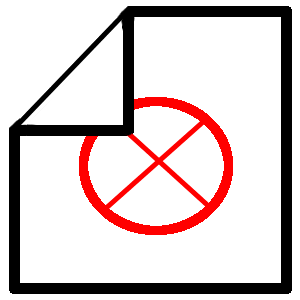
\includegraphics[width=0.2\textwidth]{dummy.png} % <- formatos PNG, JPG e PDF
	\fonte{ABNTEX, 2009\nocite{abnTeX2009}}
	\label{fig:dummy}
\end{figure}

\section{Tabelas}

Tamb\'em \'e apresentado o exemplo da Tabela~\ref{tab:correlacao}, que aparece automaticamente na lista de tabelas. Informa\c{c}\~oes sobre a constru\c{c}\~ao de tabelas no \LaTeX\ podem ser encontradas na literatura especializada~\cite{Lamport1986,Buerger1989,Kopka2003,Mittelbach2004}.

\begin{table}[!htb]
	\centering
	\caption[Exemplo de uma tabela]{Exemplo de uma tabela mostrando a correla\c{c}\~ao entre x e y.}
	\label{tab:correlacao}
	\begin{tabular}{c|c}
		\hline \SPACE
		\textbf{x} & \textbf{y} \\ \hline \SPACE
		1 & 2 \\ \hline \SPACE
		3 & 4 \\ \hline \SPACE
		5 & 6 \\ \hline \SPACE
		7 & 8 \\
		\hline 
	\end{tabular}
	\fonte{Pr\'oprio Autor.}
\end{table}

\section{Equa\c{c}\~oes}

A transformada de Laplace \'e dada na equa\c{c}\~ao~(\ref{eq:laplace}), enquanto a equa\c{c}\~ao~(\ref{eq:dft}) apresenta a formula\c{c}\~ao da transformada discreta de Fourier bidimensional\footnote{Deve-se reparar na formata\c{c}\~ao esteticamente perfeita destas equa\c{c}\~oes!}.

\begin{equation}
X(s) = \int\limits_{t = -\infty}^{\infty} x(t) \, \text{e}^{-st} \, dt
\label{eq:laplace}
\end{equation}

\begin{equation}
F(u, v) = \sum_{m = 0}^{M - 1} \sum_{n = 0}^{N - 1} f(m, n) \exp \left[ -j 2 \pi \left( \frac{u m}{M} + \frac{v n}{N} \right) \right]
\label{eq:dft}
\end{equation}

\section{Siglas e s\'imbolos}

O pacote abn\TeX\ permite ainda a defini\c{c}\~ao de siglas e s\'imbolos com indexa\c{c}\~ao autom\'atica atrav\'es dos comandos {\ttfamily \textbackslash sigla\{\}\{\}} e {\ttfamily \textbackslash simbolo\{\}\{\}}. Por exemplo, o significado das siglas\sigla{CCECOMP}{Colegiado do Curso de Engenharia de Computa\c{c}\~ao},\sigla{DAEComp}{Diretório Acad\^emico de Engenharia de Computa\c{c}\~ao} e\sigla{UEFS}{Universidade Estadual de Feira de Santana} aparecem automaticamente na lista de siglas, bem como o significado dos s\'imbolos\simbolo{$\lambda$}{comprimento de onda},\simbolo{$v$}{velocidade} e\simbolo{$f$}{frequ\^encia} aparecem automaticamente na lista de s\'imbolos. Mais detalhes sobre o uso destes e outros comandos do abn\TeX\ s\~ao encontrados na sua documenta\c{c}\~ao espec\'ifica~\cite{abnTeX2009}.

    \chapter{Fundamentação Teórica}

\section{Lógica na Filosofia e na Matemática}

De início é necessária uma definição de lógica. A lógica ou lógica clássica não foi criada, e sim caracterizada por Aristóteles (384-322 a.C.), podendo ser definida como uma ciência que estuda princípios e métodos de inferência, com o objetivo de determinar em que condições certos fatos são consequência, ou não, de outros \cite{mortari2001}.

Para o filósofo Aristóteles, o objeto da lógica é o silogismo, que é um argumento constituído de proposições das quais se infere uma conclusão, tais proposições devem seguir três princípios fundamentais \cite{zamudio2008tres}: 

\begin{itemize}
    \item \textbf{Princípio da identidade}: Indica a identidade dos seres e das coisas a partir do verbo ser, por exemplo, \textit{"A é A"}.
    \item \textbf{Princípio da não-contradição}: É impossível que um atributo pertença e não pertença ao mesmo sujeito, por exemplo, sabendo que \textit{A é A}, é impossível que \textit{A} seja \textit{não-A}.
    \item \textbf{Princípio do terceiro excluído}: Garante que não haja uma terceira possibilidade, assim duas proposições contraditórias não podem ser ambas verdadeiras em uma mesma relação, por exemplo, (\textit{\{A é x\} e \{A não é x\}}) não é verdade
\end{itemize}

O silogismo em si, trata-se de uma estrutura linguística dedutiva, baseada na existência de duas premissas e uma conclusão tirada a partir das mesmas, como demonstra o exemplo a seguir \cite{mortari2001}:

\begin{quote}\centering
    \textit{Todo gato é mamífero \\
    Miau é um gato \\
    Miau é mamífero}
\end{quote}

Essa sequência de premissas e uma conclusão é o primeiro passo para a lógica proposicional, que trata de interpretar enunciados atribuindo valores verdade às suas proposições, podendo incluir operações que permitem construir proposições complexas, como as operações de conjunção ("E"), disjunção ("OU"), implicação ("SE ... ENTÃO ...") e negação ("NÃO") \cite{flavio2010}. A tabela \ref{tab:log}, demonstra uma comparação entre a lógica clássica e a lógica proposicional, indicando um dos operadores proposicionais, o "ENTÃO".

\begin{table}[!htb]
\centering
	\caption[Comparação entre a lógica clássica no mundo real e a lógica proposicional]{Comparação entre a lógica clássica no mundo real e a lógica proposicional}
	\label{tab:log}
\begin{tabular}{c|c}
\hline \SPACE
\textbf{MUNDO REAL}                             & \textbf{PROPOSIÇÃO LÓGICA} \\ \hline \SPACE
Hoje está chovendo                              & $P$                          \\ \hline \SPACE
A rua está molhada                              & $Q$                          \\ \hline \SPACE
Se hoje está chovendo, então a rua está molhada & $P \rightarrow Q$          \\ \hline
\end{tabular}
\fonte{Próprio Autor.}
\end{table}

A lógica matemática nasce a partir da lógica proposicional em meados do século XIX, pelos tratamentos matemáticos sistemáticos de George Boole (1815 - 1864) e Augustus De Morgan (1806 - 1871), que nos permite interpretar proposições matemáticas de forma a julgá-las como verdadeiras ou falsas \cite{ferreiros2001}. Com a lógica matemática pode-se representar os operadores proposicionais em operadores lógicos para a formulação de afirmações matemáticas.


\section{Lógica de Ordem Zero e Lógica de Primeira Ordem}

A lógica proposicional contém um conjunto de fórmulas, que pode ser denominado como \simbolo{$L_\emptyset$}{Lógica de ordem zero}, também conhecido como lógica de ordem \simbolo{$\emptyset$}{Vazio}, bem como existe uma extensão da lógica proposicional que é chamada de Lógica de Primeira Ordem (\sigla{LPO}{Lógica de Primeira Ordem}). A principal diferença entre as duas é basicamente o que cada linguagem pressupõe sobre a natureza da realidade. Enquanto a $L_\emptyset$ assume que existem fatos verdadeiros ou falsos no mundo, a LPO pressupõe que as relações entre determinados objetos são válidas ou não-válidas \cite{fonseca2012logica}.

Esta seção apresenta um estudo da $L_\emptyset$ e da LPO dividindo ambos em suas abordagens semântica e sintática.

\subsection{Sintaxe da Lógica de Ordem Zero}

O primeiro passo para compreender a $L_\emptyset$, é entender os seus conectivos, sabendo que cada formula é uma proposição gerada pela concatenação de símbolos pertencentes ao alfabeto da $L_\emptyset$ que é composto pelos seguintes itens:

\begin{itemize}
    \item \textbf{Símbolos proposicionais}: $\wp = \{P, Q, R, S, P_1, P_2, ...\}$
    \item \textbf{Conectivos}: Unários e binários, demonstrados na tabela \ref{tab:cp}
    \item \textbf{Elementos de pontuação}: '(' e ')'
\end{itemize}

\begin{table}[!htb]
\centering
	\caption[Conectivos proposicionais]{Conectivos proposicionais}
	\label{tab:cp}
\begin{tabular}{c|c}
\hline \SPACE
\textbf{CONECTIVO} & \textbf{SIGNIFICADO} \\ \hline \SPACE
\simbolo{$\neg$}{Negação lógica (NÃO)}                  & "NÃO"                \\ \hline \SPACE
\simbolo{$\lor$}{Disjunção lógica (OU)}                  & "OU"                 \\ \hline \SPACE
\simbolo{$\land$}{Conjunção lógica (E)}                  & "E"                  \\ \hline \SPACE
\simbolo{$\rightarrow$}{Implicação lógica (SE...ENTÃO)}                  & "SE ... ENTÃO ..."   \\ \hline \SPACE
\simbolo{$\leftrightarrow$}{Bicondicional lógica (SE E SOMENTE SE)}                  & "SE E SOMENTE SE"    \\ \hline
\end{tabular}
\fonte{\cite{flavio2010}}
\end{table}

Assim como na língua portuguesa, na $L_\emptyset$ nem toda concatenação é válida. Os elementos da $L_\emptyset$ são chamados de fórmulas, sendo que cada formula segue um conjunto de regras para sua formação \cite{mendelson2009introduction}: 

\begin{enumerate}
    \item Todos os símbolos proposicionais são chamados de fórmulas
    \item Se $P$ é uma fórmula, então $\neg P$ também é uma fórmula
    \item Se $P$ e $Q$ são fórmulas, então ($P \lor Q$), ($P \land Q$), ($P \rightarrow Q$) e ($P \leftrightarrow Q$) também são fórmulas
\end{enumerate}

O conectivo $\neg$ também se aplica a todas as regras acima. Utilizando as mesmas de forma recursiva, com a aplicação dos parênteses quando necessário, é possível obter um conjunto infinito de fórmulas.

\subsection{Semântica da Lógica de Ordem Zero}

A semântica da $L_\emptyset$ consiste basicamente em atribuir valores verdade (verdadeiro ou falso) às fórmulas da linguagem, com o objetivo de saber se seu resultado é verdadeiro ou falso. Para realizar essa validação existem diversos métodos de inferência, tais como, tabelas-verdade, tablôs semânticos, princípio da resolução e dedução natural \cite{flavio2010}.

\subsubsection{Tabela-Verdade}

O método da tabela-verdade tem o objetivo de determinar a validade de um argumento atribuindo valores verdadeiros ou falsos para todos os símbolos proposicionais, examinando todos os casos possíveis e gerando uma visão geral de toda a fórmula, sendo que para um conjunto infinito de letras sentenciais tem-se um conjunto também infinito de valorações \cite{mortari2001}, onde cada um dos operadores lógicos gera um determinado resultado, como demonstrado na tabela \ref{tab:basic-values}.

\begin{table}[!htb]
\centering
\caption[Tabela-verdade básica]{Tabela-verdade básica}
\label{tab:basic-values}
\begin{tabular}{c|c|c|c|c|c|c|c}
\hline
\textbf{P} & \textbf{Q} & \textbf{$\neg$P} & \textbf{$\neg$Q} & \textbf{$\mathbf{P \lor Q}$} & \textbf{$\mathbf{P \land Q}$} & \textbf{$\mathbf{P \rightarrow Q}$} & \textbf{$\mathbf{P \leftrightarrow Q}$} \\ \hline
V          & V          & F                & F                & V            & V                             & V                          & V                                     \\ \hline
V          & F          & F                & V                & V            & F                             & F                          & F                                     \\ \hline
F          & V          & V                & F                & V            & F                             & V                          & F                                     \\ \hline
V          & F          & V                & V                & F            & F                             & V                          & V                                     \\ \hline
\end{tabular}
\fonte{\cite{mortari2001}}
\end{table}

Um exemplo de tabela-verdade simples pode ser dado a partir da fórmula $(\neg A \land \neg B) \rightarrow \neg A $, atribuindo valores verdade para A e/ou B. Partindo desses valores pode-se construir a tabela \ref{tab:tva}.

\begin{table}[!htb]
\centering
\caption[Tabela-verdade para a expressão $\mathbf{(\neg A \land \neg B) \rightarrow \neg A }$]{Tabela-verdade para a expressão $\mathbf{(\neg A \land \neg B) \rightarrow \neg A }$}
\label{tab:tva}
\begin{tabular}{c|c|c|c|c}
\hline
\textbf{A} & \textbf{B} & $\mathbf{\neg A}$ & $\mathbf{\neg A \land \neg B}$ & $\mathbf{(\neg A \land \neg B) \rightarrow \neg A}$ \\ \hline
V          & V          & F          & F          & V          \\ \hline
F          & V          & V          & V          & V          \\ \hline
V          & F          & F          & F          & V          \\ \hline
F          & F          & V          & F          & V          \\ \hline
\end{tabular}
\fonte{\cite{mortari2001}}
\end{table}

Quando se tem uma fórmula onde todas as suas valorações são verdadeiras, a mesma é denominada tautologia.

\subsection{Sintaxe da Lógica de Primeira Ordem}

\subsubsection{Símbolos}

A LPO faz a suposição de que o mundo é constituído de objetos com certas propriedades ou relações entre eles, onde os objetos podem ser definidos em função de outros objetos e suas relações podem ser verdadeiras ou falsas. A linguagem geral do cálculo de predicados de primeira ordem é formada por símbolos lógicos e não-lógicos \cite{mortari2001}, que devidamente agrupados formam os axiomas. 

\begin{itemize}
    \item \textbf{Símbolos lógicos}: 
        \begin{itemize}
            \item \textit{Símbolos de constantes}: um conjunto enumerável de nomes específicos de objetos no domínio do discurso.
            \item \textit{Símbolos de predicados}: um conjunto enumerável de símbolos que representam relações.
        \end{itemize}
        Ambos são representados por letras maiúsculas (\textit{A, B, X, Y}, etc)
        
    \item \textbf{Símbolos não-lógicos}:
        \begin{itemize}
            \item \textit{Variáveis}: Nomeiam um conjunto de objetos, geralmente representadas por letras minúsculas (\textit{x}, \textit{y}, \textit{z}, etc).
            \item \textit{Operadores}: Incluem os conectivos unários e binários demonstrados na tabela \ref{tab:cp}.
            \item \textit{Quantificadores}: O quantificador universal $\forall$ e o quantificador existencial $\exists$.
            \item \textit{Sinais de pontuação}:  '(' e ')'.
        \end{itemize}
\end{itemize}

\subsubsection{Fórmulas}

A partir do conjunto acima de símbolos, podem ser construídas as fórmulas que definem a composição de uma proposição, por exemplo, considerando a afirmação "x é um filósofo", é possível escolher um símbolo de predicado para representar o fato de ser um filósofo, podendo ser F por exemplo. Em seguida infere-se que x pode ser qualquer indivíduo, esse é uma variável, podendo ser 'a':

\begin{itemize}
    \item \textit{F}: 'x é um filósofo'
    \item \textit{a}: Aristóteles
\end{itemize}

A partir dos dados acima é possível construir uma fórmula que representa que "Aristóteles é um filósofo" usando a notação '\textit{Fa}', essa é a formula mais simples que se tem na LPO, sendo denominada fórmula atômica \cite{mortari2001}. Não existe uma convenção que defina a ordem de construção de uma fórmula atômica, porém é necessário que se mantenha uma homogeneidade na construção das fórmulas. Adicionando mais variáveis, é possível construir sentenças mais complexas usando somente fórmulas atômicas, se for acrescentado que Platão também é um filósofo, representando o mesmo pela letra '\textit{p}', a fórmula \textit{Fpa} representa que Platão e Aristóteles são filósofos.

Caso uma sentença tenha mais de uma fórmula atômica, a mesma é denominada de fórmula molecular, nesse caso entra o uso dos conectivos (tabela \ref{tab:cp}) para realizar a composição de uma fórmula. Tomando como base a fórmula \textit{Fpa} citada anteriormente, pode-se adicionar mais uma fórmula atômica, por exemplo:

\begin{itemize}
    \item \textit{M}: 'x é um matemático'
    \item \textit{f}: Fourier
\end{itemize}

Assim pode-se construir a fórmula molecular que infere que Platão e Aristóteles são filósofos e Fourier é matemático, da seguinte maneira, sendo os parênteses facultativos nesse caso:

\begin{quote}\centering
    (\textit{Fpa} $\land$ \textit{Mf})
\end{quote}

Como afirmado por \citeonline{mendelson2009introduction}, citado anteriormente na seção 2.2.1, usando os conectivos proposicionais podem se formar diversas fórmulas onde \textit{P} e \textit{Q} podem ser tanto fórmulas atômicas quanto moleculares.

Segundo \citeonline{mortari2001}, Uma linguagem de primeira ordem é qualquer subconjunto da linguagem geral do cálculo de predicados de primeira ordem (\sigla{CQC}{Cálculo Quantificacional Clássico de Primeira Ordem}) que inclua todos os símbolos lógicos e pelo menos uma constante de predicado. Essa informação infere que é possível construir fórmulas se dispuser de pelo menos um símbolo de predicado.

Para fórmulas moleculares um pouco mais complexas, pode-se usar parênteses como auxiliares, como no exemplo dado por \citeonline{mortari2001}, "Salma Hayek é morena, mas Claudia Schiffer e Cameron Díaz não o são". Essa expressão pode ser agrupada com colchetes e reescrita com outras palavras para facilitar o seu entendimento, como [Salma Hayek é morena] mas [Claudia Schiffer não é morena e Cameron Díaz não é morena]. Considerando M como "x não é morena", os indivíduos como \textit{s}, \textit{c} e \textit{d} respectivamente, usando os parênteses de maneira correta obtém-se a fórmula $(Ms \land (\neg Mc \land \neg Md))$.

Para fórmulas ainda mais complexas, pode-se usar os quantificadores universal (\simbolo{$\forall$}{Para todo}) e existencial (\simbolo{$\exists$}{Existe}), como no exemplo dado por \citeonline{mendelson2009introduction}, \textit{"Qualquer amigo de Martin é amigo de John"}, usando o quantificador universal, considerando as varáveis \textit{m} e \textit{j} para os indivíduos respectivamente e F como "x é amigo", é construída a fórmula $\forall x (Fxm \rightarrow Fxj)$. Da mesma forma pode-se elaborar um exemplo com o quantificador existencial, como \textit{"Algumas pessoas são amigas de Martin e John"}, formulado como: $\exists x (Fxm \land Fxj)$.

\subsubsection{Formas básicas de proposição categórica}

De forma geral, várias sentenças de estrutura mais complexa podem ser reduzidas às formas básicas de proposição categórica (tabela \ref{tab:basic}), porém há muitos exemplos que não se encaixam nesse padrão e devem ser cuidadosamente analisados para um correto resultado \cite{mortari2001}.

\begin{table}[!htb]
\centering
	\caption[Formas básicas de proposição categórica]{Formas básicas de proposição categórica}
	\label{tab:basic}
\begin{tabular}{c|c}
\hline \SPACE
Todo A é B                  & $\forall x (Ax \rightarrow Bx)$                \\ \hline \SPACE
Nenhum A é B                & $\forall x (Ax \rightarrow \neg Bx)$                 \\ \hline \SPACE
Algum A é B                  & $\exists x (Ax \land Bx)$                  \\ \hline \SPACE
Algum A não é B                  & $\exists x (Ax \land \neg Bx)$   \\ \hline
\end{tabular}
\fonte{\cite{mortari2001}}
\end{table}

\subsection{Semântica da Lógica de Primeira Ordem}

De maneira análoga a $L_\emptyset$, para a LPO o estudo da semântica é feito realizando a atribuição de valores verdade onde tais valores são destinados às sentenças moleculares, para então realizar a interpretação desses valores na fórmula geral, definindo suas relações. Isso permite a definição de consequência lógica (\simbolo{$\models$}{Consequência lógica}), denotado por $\Gamma \models \alpha$, cujo significado segundo \citeonline{mortari2001} é que se $\Gamma$ é um conjunto de fórmulas, e \simbolo{$\alpha$}{Letra grega Alfa} uma fórmula, dizemos que $\alpha$ é uma consequência lógica de \simbolo{$\Gamma$}{Letra grega Gama} se e somente se todo modelo de $\Gamma$ é também modelo de $\alpha$. Em outras palavras, segundo \citeonline{Tannen2009}, a sentença $\alpha$ é verdadeira em qualquer estrutura na qual as sentenças do conjunto $\Gamma$ são verdadeiras.

\subsubsection{Validade e tabelas-verdade}

As fórmulas podem ser classificadas em três tipos:

\begin{itemize}
    \item \textbf{Tautológicas}: Verdadeiras em todas as valorações.
    \item \textbf{Contradições}: Falsas em todas as valorações.
    \item \textbf{Contingências}: Verdadeiras em ao menos uma e falsas em ao menos uma valoração.
\end{itemize}

A partir do conceito de tautologia, pode-se definir um novo conceito para a LPO, o de fórmula válida, que denota uma fórmula verdadeira em toda e qualquer estrutura \cite{mortari2001}. Tautologias funcionam de maneira eficaz na $L_\emptyset$, porém na LPO verifica-se que nem todas as fórmulas válidas são tautologias. 

Tomando o seguinte exemplo com duas fórmulas elementares: $\forall xPx \rightarrow Pa$, apesar de ser uma fórmula válida, na tabela \ref{tab:tautologia}, vemos que ela não é uma tautologia, isso acontece porque tabelas-verdade não conseguem lidar bem com quantificadores, pois numa fórmula como $\forall xPx$ por exemplo, é impossível obter o seu valor, visto que tem um universo infinito de casos possíveis. Com isso existem outros métodos eficazes de mostrar a validade de uma estrutura na LPO, alguns deles serão citados a seguir.

\begin{table}[!htb]
\centering
	\caption[Tabela-verdade para uma fórmula válida]{Tabela-verdade para uma fórmula válida}
	\label{tab:tautologia}
\begin{tabular}{c|c|c}
\hline \SPACE
\textbf{$\forall xPx$} & \textbf{$Pa$} & \textbf{$\forall xPx \rightarrow Pa$} \\ \hline \SPACE
V                  & V        &   V     \\ \hline \SPACE
F                  & V           &  V    \\ \hline \SPACE
V                  & F            &   F   \\ \hline \SPACE
F                  & F  &  V \\ \hline
\end{tabular}
\fonte{\cite{mortari2001}}
\end{table}

\subsection{Tablôs Semânticos}

Também conhecido como árvores de refutação, o método de inferência por tablôs semânticos permite mostrar a validade ou invalidade de um fórmula, ou determinar se alguma fórmula é consequência lógica, ou não, de algum conjunto de fórmulas usando um procedimento de prova \cite{mortari2001}. Esse é um dos métodos ideais para lidar com a lógica de primeira ordem, pois consegue realizar validações com base nos quantificadores universal e existencial. 

Tomando como exemplo a fórmula $\forall xPx \rightarrow Pa$ citada anteriormente, pode-se interpreta-la como: se é verdade que todos são matemáticos, então é verdade que Fourier é matemático. Mesmo sabendo que é uma expressão verdadeira, o passo inicial é assumir que a expressão é falsa na primeira linha do tablô, e seguir os passos de comparação com o auxílio da tabela \ref{tab:basic-values}:

\begin{quote}\centering
    $\checkmark$ \textbf{F} $\forall xPx \rightarrow Pa$ \\
    \textbf{V} $\forall xPx$ \\
    \textbf{F} $Pa$
\end{quote}

Partindo para a segunda fórmula, pode-se concluir que se todos são matemáticos então $Pa$, $Pb$, $Pc$ e os demais são matemáticos, logo $Pa$ é verdadeiro, finalizando o tablô da seguinte maneira: 

\begin{quote}\centering
    $\checkmark$ \textbf{F} $\forall xPx \rightarrow Pa$ \\
    \textbf{V} $\forall xPx$ \\
    \textbf{F} $Pa$ \\
    \textbf{V} $Pa$ \\
    X
\end{quote}

\subsection{Dedução Natural}

A Dedução Natural é um sistema de prova que permite extrair conclusões a partir de um conjunto de premissas, que são fórmulas de uma lógica construídas de acordo com as regras de formação da linguagem. Isso nos permite inferir fórmulas a partir de outras fórmulas, por meio de regras denominadas regras de inferência. Ao aplicar essas regras em sucessão, podemos tirar uma conclusão a partir de um conjunto de premissas, que pode servir como premissa na obtenção de novas conclusões e assim sucessivamente \cite{huth2004logic}.

Uma dedução é construída inicialmente listando as premissas que estão ao nosso dispor e uma outra fórmula chamada de conclusão, que é o objetivo a ser atingido. Após isso podem ser aplicadas regras de inferência que permitem acrescentar uma nova linha à essa lista, contendo uma fórmula que é o resultado da aplicação da regra às fórmulas anteriores \cite{mortari2001}. Ao aplicar as regras de inferência a essas fórmulas, pode-se eventualmente obter a conclusão. Tomando \simbolo{$\phi$}{Letra graga Phi} como a lista de fórmulas e \simbolo{$\psi$}{Letra grega Psi} como a fórmula de conclusão, isso pode ser denotado por:

\begin{quote}\centering
    $\phi_1, \phi_2, ..., \phi_n \models \psi $
\end{quote}

\subsubsection{Regras de inferência diretas}

São as regras que regulam quais fórmulas podem ser inferidas a partir de outras fórmulas (figura \ref{fig:diretas}).

\begin{figure}[!htb]
	\centering
	\caption[Regras de inferência diretas]{Regras de inferência diretas.}
	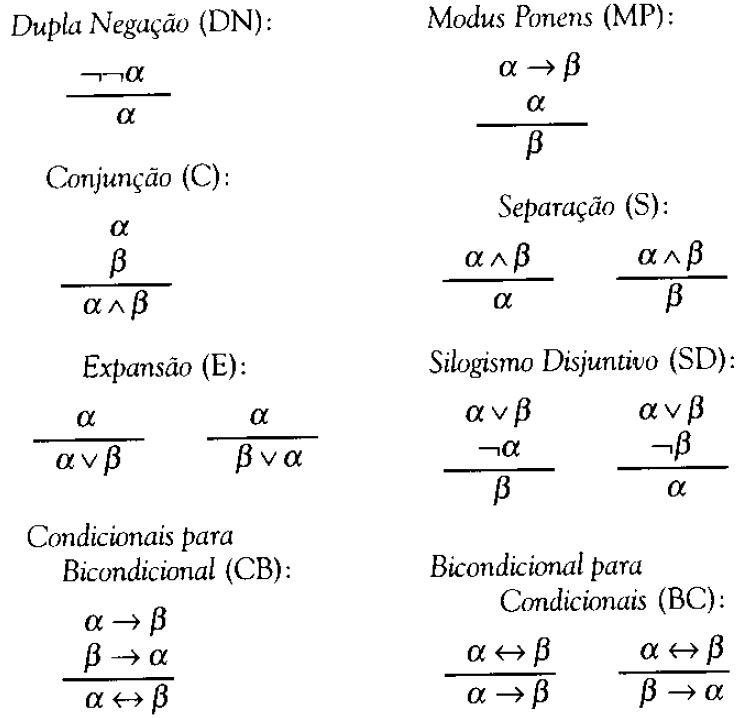
\includegraphics[width=0.6\textwidth]{diretas.png}
	\fonte{MORTARI, 2001\nocite{mortari2001}}
	\label{fig:diretas}
\end{figure}

\subsubsection{Regras de inferência hipotéticas}

Exigem o uso de hipóteses, usadas para os operadores não citados nas regras diretas, são as regras de redução ao absurdo e regra de prova condicional (figura \ref{fig:hip}). Na regra de redução ao absurdo (\sigla{RAA}{Regra de redução ao absurdo}), a partir de uma hipótese $\alpha$, deriva-se uma contradição $\beta \land \neg \beta$, então pode-se descartar $\alpha$ e introduzir $\neg \alpha$ na derivação. Na regra de prova condicional (\sigla{RPC}{Regra de prova condicional}), a partir de uma hipótese $\alpha$ que deriva uma fórmula \simbolo{$\beta$}{Letra grega Beta}, pode-se descartar $\alpha$ e introduzir $\alpha \rightarrow \beta$ na derivação \cite{mortari2001}.

\begin{figure}[!htb]
	\centering
	\caption[Regras de inferência hipotéticas]{Regras de redução ao absurdo e regra de prova condicional, respectivamente.}
	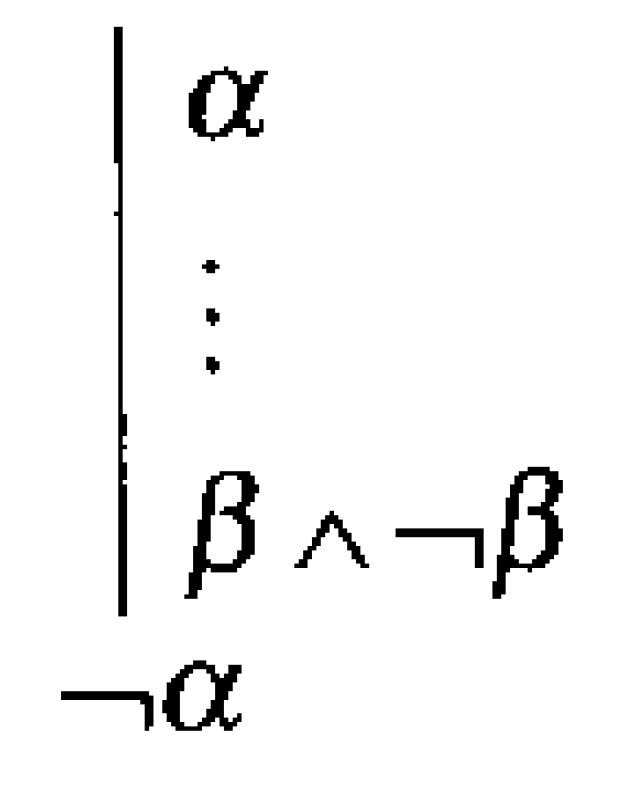
\includegraphics[width=0.15\textwidth]{raa.png}
	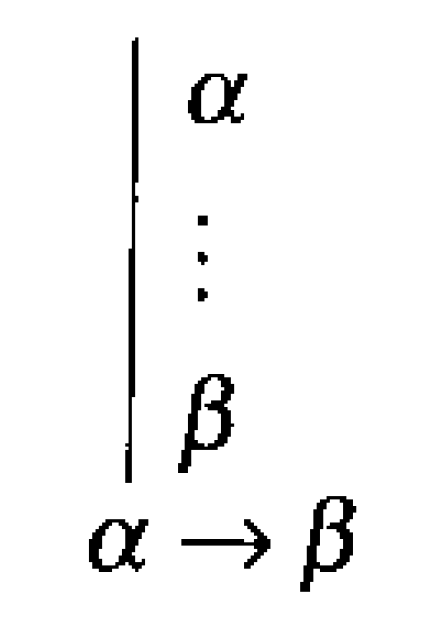
\includegraphics[width=0.15\textwidth]{rpc.png}
	\fonte{MORTARI, 2001\nocite{mortari2001}}
	\label{fig:hip}
\end{figure}

\subsubsection{Regras de inferência derivadas}

Podem ser provadas a partir das outras regras, de modo que tudo que pode ser feito com uma regra derivada, também pode ser feito usando as regras iniciais, mostrando que uma regra derivada é uma maneira de abreviar parte de uma dedução, facilitando o procedimento. a figura \ref{fig:derivadas} demonstra algumas dessas regras.

\begin{figure}[!htb]
	\centering
	\caption[Algumas regras de inferência derivadas]{Algumas regras de inferência derivadas.}
	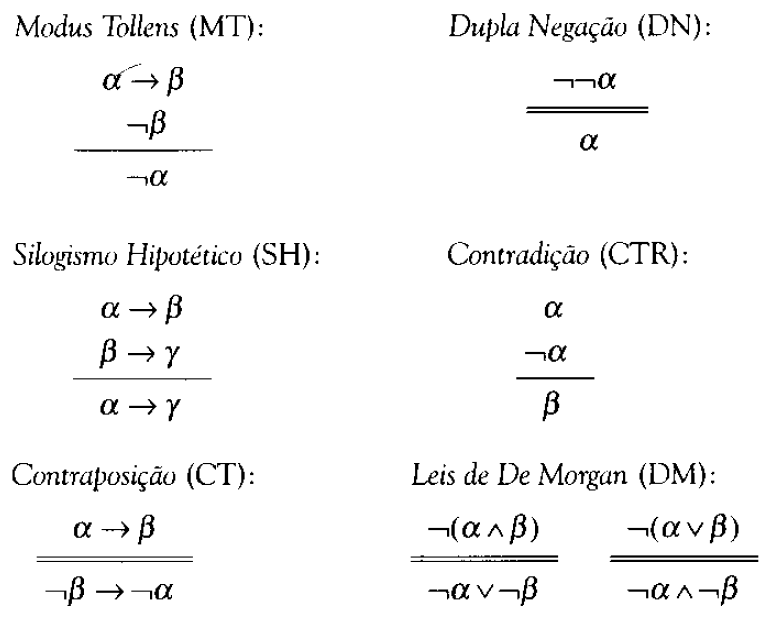
\includegraphics[width=0.6\textwidth]{derivadas.png}
	\fonte{MORTARI, 2001\nocite{mortari2001}}
	\label{fig:derivadas}
\end{figure}

\subsubsection{Regras para quantificadores}

Completam todo o conjunto de regras da dedução natural, e são usadas para lidar com os quantificadores universal e existencial, são quatro regras, sendo elas as regras de eliminação e introdução dos quantificadores universal (figura \ref{fig:universal}) e existencial (figura \ref{fig:existencial}).

\begin{figure}[!htb]
	\centering
	\caption[Regras para o quantificador universal]{Regras para o quantificador universal.}
	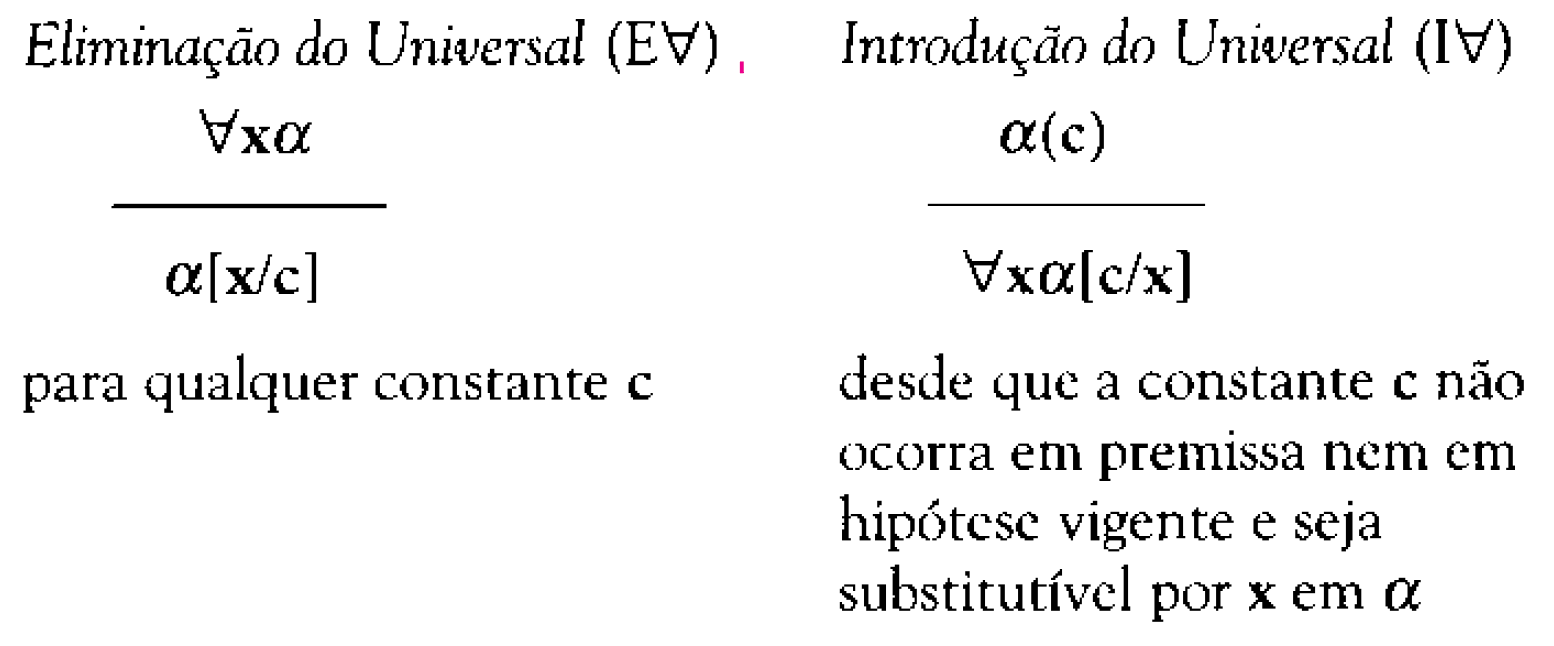
\includegraphics[width=0.6\textwidth]{universal.png}
	\fonte{MORTARI, 2001\nocite{mortari2001}}
	\label{fig:universal}
\end{figure}

\begin{figure}[!htb]
	\centering
	\caption[Regras para o quantificador existencial]{Regras para o quantificador existencial.}
	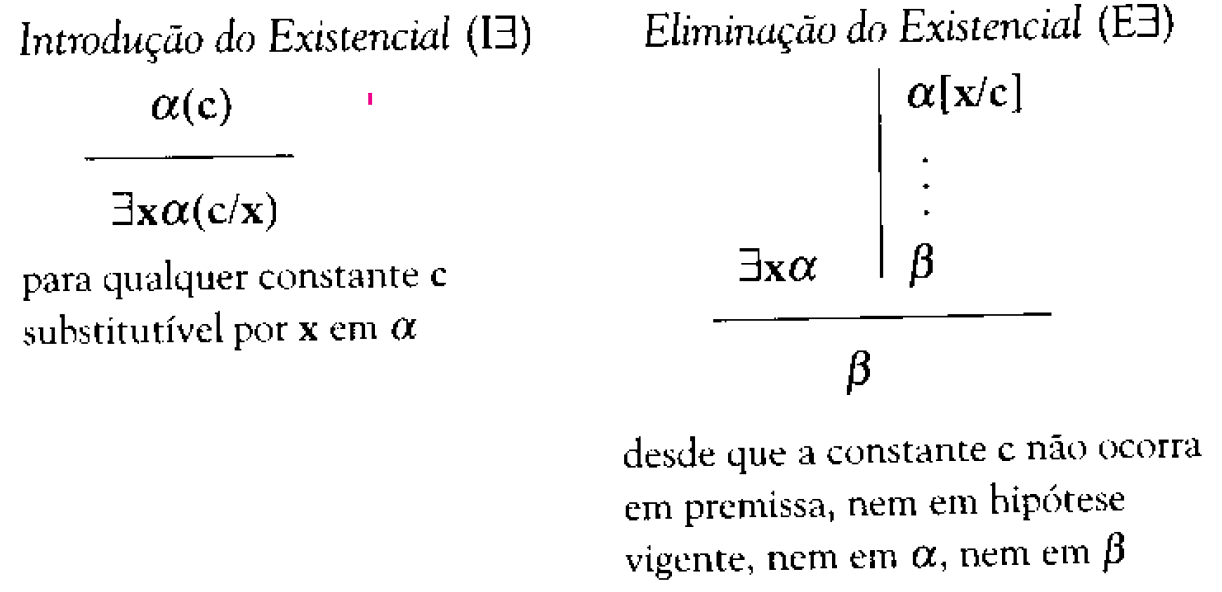
\includegraphics[width=0.6\textwidth]{existencial.png}
	\fonte{MORTARI, 2001\nocite{mortari2001}}
	\label{fig:existencial}
\end{figure}

\section{Problema da Satisfatibilidade Booleana}

O problema da satisfatibilidade booleana (SAT) trata da verificação da existência de uma atribuição de valores verdadeiro ou falso que torne em verdadeira uma fórmula booleana expressa em forma normal conjuntiva (\sigla{FNC}{Forma Normal Conjuntiva}). Esse problema ocupa um papel fundamental na ciência da computação teórica, especialmente no contexto da teoria de complexidade de problemas. Diante de uma fórmula booleana, o desafio é determinar se há uma combinação de valores para suas variáveis que faça com que a expressão seja satisfeita \cite{el2016computational}.

O SAT foi o primeiro problema a ser demonstrado como NP-completo \cite{cook2023complexity}, ou seja, qualquer problema em \sigla{NP}{Tempo polinomial não determinístico} pode ser reduzido a SAT em tempo polinomial: para todo problema \( L \) em NP, existe uma função computável polinomialmente que, dada uma instância \( w \) de \( L \), constrói uma fórmula em FNC satisfazível se, e somente se, \( w \in L \). A prova técnica envolve codificar o funcionamento de uma máquina de \textit{Turing} não determinística na estrutura lógica da fórmula, de modo que satisfazer a fórmula equivale a simular a aceitação da máquina \cite{Cook_Levin-AFP}. Toda a importância solução do SAT, alavancou o desenvolvimento de algoritmos otimizados para resolve-lo, se tornando um objetivo crucial na área de pesquisa em algoritmos e complexidade. 

Na prática, apesar de sua complexidade, muitos exemplos do SAT são tratáveis por \textit{solvers} contemporâneos, que combinam algoritmos como \sigla{DPLL}{Davis–Putnam–Logemann–Loveland} (Davis–Putnam–Logemann–Loveland), \sigla{CDCL}{Conflict‑Driven Clause Learning} (Conflict‑Driven Clause Learning) e busca local. Além disso, há pesquisas recentes aplicando técnicas de aprendizado de máquina para melhorar heurísticas \textit{solver} \cite{guo2023machine}.

\subsection{O Problema MAX-SAT}

O MAX-SAT é uma extensão do clássico problema de SAT, onde o objetivo não é apenas encontrar uma atribuição que satisfaça todas as cláusulas de uma fórmula na FNC, mas sim a que maximiza o número de cláusulas satisfeitas, caracterizando o seu nome em tradução livre para o português como Satisfatibiliade Máxima. Formalmente, dada uma fórmula \( \varphi = C_1 \land C_2 \land \cdots \land C_k \) composta por cláusulas \( C_i \), busca-se uma atribuição \textit{booleana} \( A \) que maximize a quantidade de cláusulas para as quais \( A(C_i) = \textit{true} \) \cite{el2016computational}. 

Considerando que a quantidade de cláusulas tem no máximo 2 literais cada, temos a versão restrita conhecida como MAX‑2‑SAT e assim sucessivamente para \textit{n} literais. Apesar dessa simplificação estrutural, essa variante continua NP-completa na versão de decisão (isto é, determinar se existe uma atribuição que satisfaça pelo menos \textit{k} cláusulas). A formulação geral do MAX‑SAT também pertence à classe NP-completo, conforme demonstrado em estudos clássicos de complexidade \cite{krentel1986complexity}.

Esse problema é fundamental tanto teoricamente quanto na prática. Ele aparece em domínios como, verificação de hardware e software, roteamento de satélites, \textit{timetabling}, entre outros tópicos da Ciência da Computação e Engenharia Elétrica. Consequentemente, há intenso esforço acadêmico voltado a \textit{solvers} que sejam capazes de resolver grandes conjuntos de exemplos do MAX-SAT, bem como a heurísticas e algoritmos aproximados \cite{biere2009handbook}. 

\subsection{Transição de Fase}

A transição de fase em problemas SAT é um fenômeno observado quando se estuda o comportamento de instâncias aleatórias de fórmulas booleanas em função da razão entre cláusulas e variáveis. Especificamente, à medida que aumentamos essa razão, existe um ponto crítico no qual a probabilidade de que uma fórmula seja satisfatível cai abruptamente de quase 1 para quase 0, esse ponto é conhecido como limiar de transição de fase e tem sido intensamente estudado por sua relevância teórica e prática em ciência da computação, especialmente na análise de desempenho de algoritmos de resolução de SAT \cite{cheeseman1991really}. 

Estudos realizados por \citeonline{mitchell1992hard} observaram que instâncias de problemas SAT aleatórios são mais difíceis de resolver quando a razão entre o número de cláusulas e o número de variáveis se aproxima de um valor crítico. Abaixo desse valor, a maioria das instâncias é satisfazível e fácil de resolver, enquanto acima dele, a maioria é insatisfazível e também relativamente fácil de provar sua insatisfatibilidade.

Um estudo realizado por \citeonline{crawford1996experimental}, demonstrou graficamente a relação entre a porcentagem de satisfatibilidade e a dificuldade de um problema \textit{3-SAT} para 200 variáveis aleatórias, considerando a razão $\alpha$ de cláusula/variável. A figura \ref{fig:phase-graph} exemplifica o ponto de transição de fase graficamente, onde uma linha mostra a porcentagem satisfazível e a outra mostra a dificuldade do problema. A dificuldade do problema atinge o pico na região onde a porcentagem satisfazível cai repentinamente de quase cem por cento para quase zero. À medida que $\alpha$ aumentava de 0 para 4,3, o problema começava fácil, exigindo um pequeno número de lançamentos para encontrar uma solução, para difícil, exigindo significativamente mais lançamentos, e então para fácil novamente após $\alpha$ = 4,3 \cite{qasem2009sat}.

\begin{figure}[!htb]
	\centering
	\caption[Demonstração do ponto de transição de fase]{Demonstração do ponto de transição de fase.}
	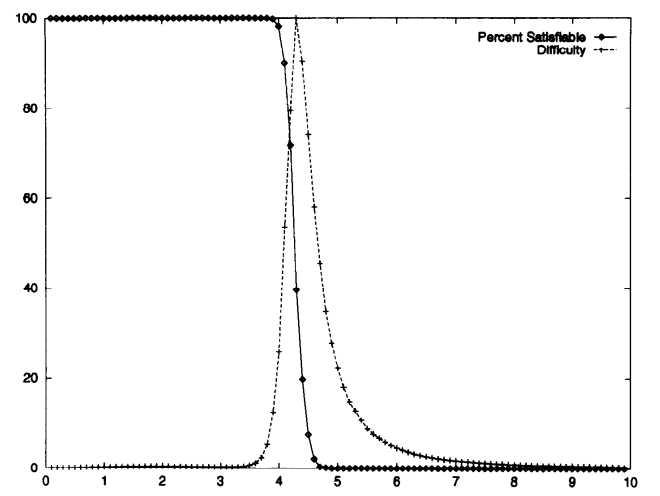
\includegraphics[width=0.6\textwidth]{phase-graph.png}
	\fonte{CRAWFORD; AUTON, 1996\nocite{crawford1996experimental}}
	\label{fig:phase-graph}
\end{figure}

No contexto do MAX-SAT a transição de fase também se manifesta, embora de forma mais complexa. Em vez de um comportamento binário, o foco está na fração de cláusulas que podem ser satisfeitas à medida que a razão $\alpha$ varia. Estudos como os de \citeonline{monasson1999determining} mostraram que existe uma mudança abrupta no comportamento estatístico dessas instâncias, especialmente no número esperado de cláusulas satisfeitas e na estrutura das soluções. Essa mudança tem implicações diretas na tratabilidade dos problemas, onde quando próximos à transição de fase, instâncias tendem a ser mais difíceis de resolver, demandando mais tempo computacional, tanto por algoritmos exatos quanto por heurísticas.

Compreender a transição de fase no MAX-SAT é essencial para o desenho de algoritmos mais eficientes e para a análise de complexidade média. O estudo desses fenômenos indica que as regiões de transição carregam informações cruciais sobre a estrutura do espaço de soluções e o comportamento típico de instâncias difíceis, abrindo caminho para avanços tanto teóricos quanto práticos na computação.
 
\subsection{SAT Solvers}

\textit{SAT solvers} são ferramentas computacionais desenvolvidas para solucionar problemas SAT, e tornaram-se essenciais em áreas como verificação formal, inteligência artificial e otimização. \textit{Solvers} para MAX-SAT adaptam técnicas dos \textit{SAT Solvers}, incorporando estratégias específicas para balancear eficiência e qualidade da solução, esses \textit{solvers} buscam encontrar a atribuição de variáveis que maximiza o número de cláusulas satisfeitas, ao invés de simplesmente verificar se todas podem ser satisfeitas simultaneamente.

Pesquisas recentes têm se concentrado em adaptar e otimizar algoritmos do SAT para resolver eficientemente exemplos do MAX-SAT, explorando técnicas como \textit{branch-and-bound}, relaxações lineares e aprendizado de cláusulas. Avanços na codificação e nas heurísticas específicas para o MAX-SAT têm levado a melhora do desempenho dos \textit{solvers}, tornando-os em ferramentas práticas para problemas reais em diversas áreas da computação \cite{li2007new}.
    \chapter{Revisão Bibliográfica Sistemática}

Para dar início à feitura de um trabalho científico, é de suma importância a realização de uma Revisão Bibliográfica Sistemática (\sigla{RBS}{Revisão Bibliográfica Sistemática}) de trabalhos correlatos ao tema em pesquisa, reunindo-se fontes confiáveis para a confecção do novo trabalho. Esse processo visa a alguma tendência de inovação, para enriquecer o estado da arte.

Neste capítulo será discriminado o passo a passo da realização da RBS, desde a construção de uma questão de pesquisa baseada no tema, até a pormenorização da informação construída.

\section{Questão de Pesquisa} 

A RBS foi iniciada tomando como base a seguinte questão de pesquisa: "A que conclusões comparativas pode-se chegar, a partir de uma análise do fenômeno de transição de fase, em soluções de exemplos do Problema da Satisfatibilidade Booleana (\sigla{SAT}{Problema da Satisfatibilidade Booleana})?".

\section{Processo de Revisão Bibliográfica Sistemática}

Esta RBS foi feita em meio digital, com o auxílio de bases de pesquisa confiáveis para a busca de referências e a verificação indireta de outras, a ser encontradas nessas, que fossem consideradas relevantes.

\subsection{Base de Pesquisa}

Para se obterem mais resultados e o uso de um método de caracterização da qualidade dos itens encontrados, foram utilizadas duas bases de pesquisa para esta RBS, o \textit{Google} Acadêmico e o \textit{IEEE Xplore}.

\subsubsection{Google Acadêmico}

Trata-se de uma ferramenta lançada pelo \textit{Google} em 2004, com o objetivo de ser um mecanismo de pesquisa de livre acesso à comunidade, para indexar textos da literatura acadêmica, sejam eles livros, revistas, patentes, teses, dissertações, entre outros. Um dos recursos mais úteis do \textit{Google} Acadêmico é a possibilidade de usar operadores booleanos e operadores de busca para refinar uma pesquisa na ferramenta. A partir dessa funcionalidade por exemplo, pode-se criar uma query de busca específica de apenas partes de um texto dentro do resultado, podendo ser uma lista de diferentes partes usando o operador booleano OR. Além dessas funções pode-se destacar também a possibilidade de se realizarem filtragens de uma pesquisa por um período específico de tempo, por idioma ou por relevância. O \textit{Google} Acadêmico ao encontrar um texto exibe de imediato informações úteis sobre o mesmo, como o autor, a quantidade de citações, outros textos relacionados, onde e quando foi publicado, além de ser fornecida a maneira correta de realizar a sua citação em vários padrões.

Para as pesquisas realizadas foi usado o operador de busca \textit{intitle}, que mostra resultados contendo a palavra-chave ou frase especificada dentro do título da página, inclusive em diversas combinações diferentes.

\subsubsection{IEEE Xplore}

É um banco de dados para busca de artigos, anais de conferências, normas técnicas e outros materiais relacionados diretamente às áreas de engenharia elétrica e eletrônica e ciências da computação. Criado pelo Instituto de Engenheiros Eletricistas e Eletrônicos (\sigla{IEEE}{Instituto de Engenheiros Eletricistas e Eletrônicos}) em 2000, contém material publicado principalmente por afiliados do IEEE e outras editoras parceiras.

Assim como o \textit{Google} Acadêmico, o \textit{IEEE Xplore} também fornece vários métodos de aplicar as buscas, com o uso de operadores específicos tendo a finalidade de retornar melhores resultados. Além dos operadores booleanos AND, OR e NOT, o \textit{IEEE Xplore} possui uma série de \textit{Data Fields}, que identificam partes específicas de um documento com a finalidade de limitar uma pesquisa somente a essas partes, por exemplo, existe o campo \textit{Document Title}, que busca somente registros encontrados nos títulos dos documentos. 

A possibilidade de filtragem por data e relevância aliado às ferramentas de pesquisa avançada tornam o \textit{IEEE Xplore} uma ótima base de dados para enriquecimento da RBS.

\subsection{Queries de Busca}

Como as primeiras buscas foram realizadas utilizando o \textit{Google} Acadêmico, foram elaboradas as \textit{queries} de busca abaixo, usando somente do operador \textit{intitle}, que busca por resultados que obrigatoriamente devem ter determinado termo no título, nesse caso o termo SAT deve estar presente no título de todos os artigos encontrados na busca, enquanto o restante da \textit{query} pode estar localizado tanto no título quanto no conteúdo do documento.

\begin{itemize}
   \item intitle:SAT solver phase transition
   \item intitle:SAT solver phase transition analysis
\end{itemize} 

Na elaboração das \textit{queries} de busca para o IEEE Xplore, foi tido como base o mesmo critério usado para o Google Acadêmico, onde o termo SAT deve estar obrigatoriamente presente no título do documento. para construir a query de busca específica para o IEEE Xplore foi utilizada a ferramenta \textit{Command Search} do mesmo, que permite agrupar os operadores disponíveis para a busca avançada com o texto que deve ser pesquisado, criando uma \textit{query} de busca. Alguns dos operadores que podem ser usados estão listados na tabela \ref{table:ieeexplore_opeartors}.

\begin{table}[!htb]
\centering
\caption{Exemplos de operadores do IEEE Xplore}
    \begin{tabular}{|p{3cm}|P{10cm}|}
    \hline
    \rowcolor[HTML]{C0C0C0} 
    \textbf{Operador}     & \textbf{Descrição}                                                                                                                                                              \\ \hline
    Document Title        & Título de um documento individual (artigo de periódico, artigo de conferência, padrão, capítulo de livro ou curso).                                                             \\ \hline
    Full Text \& Metadata & Full Text refere-se ao texto de um artigo, norma, etc. Metadata são as informações detalhadas que descrevem o texto completo, como nomes dos autores, data de publicação e DOI. \\ \hline
    AND                   & Para x AND y, corresponde ambas as expressões x e y                                                                                                                             \\ \hline
    OR                    & Para x OR y, corresponde à expressão x ou y ou ambas                                                                                                                            \\ \hline
    \end{tabular}
\label{table:ieeexplore_opeartors}
\end{table} 


 Nos primeiros testes de busca foi utilizada a query (("Document Title":SAT) AND ("Full Text \& Metadata":"solver phase transition")), utilizando também da precedência de parenteses para o correto reconhecimento da query, porém esta trouxe pouquíssimos resultados, pois o operador \textit{"Full Text \& Metadata"} considera todo o texto indicado, na ordem em que está escrito. Nesse caso foi necessário o uso dos operadores AND e OR para obter os resultados de forma semelhante às \textit{queries} usadas para o Google Acadêmico, resultando nas seguintes \textit{queries}:

    \begin{itemize}
        \item (("Document Title":SAT) AND ("Full Text \& Metadata":solver OR "Full Text \& Metadata":"phase transition"))
        \item (("Document Title":SAT) AND ("Full Text \& Metadata":solver OR "Full Text \& Metadata":"phase transition" OR "Full Text \& Metadata":analysis))
    \end{itemize}

Conforme as \textit{queries} de busca acima, utilizando do operador "Full Text \& Metadata", é realizada uma busca das expressões 'solver', 'phase transition' e 'analysis' separadamente em todo o conteúdo do documento, resultando assim uma quantidade satisfatórias de resultados como indicado.

Com uma quantidade satisfatória de resultados para cada \textit{query}, foi verificado que as mesmas ajudaram bastante gerando uma quantidade de resultados satisfatória na busca, conforme demonstra as tabelas \ref{table:gs_result} e \ref{table:ieee_result}.

\begin{table}[!htb]
\centering
\caption{Quantidade de resultados nas buscas usando Google Acadêmico}
\begin{tabular}{|l|c|}
\hline
\rowcolor[HTML]{C0C0C0} 
\textbf{\textit{Query} de Busca}                      & \textbf{Quantidade de Itens} \\ \hline
\textit{intitle:SAT solver phase transition}          & 751                          \\ \hline
\textit{intitle:SAT solver phase transition analysis} & 620                          \\ \hline
\end{tabular}\label{table:gs_result}
\end{table}

\begin{table}[!htb]
\centering
\caption{Quantidade de resultados nas buscas usando IEEE Xplore}
\begin{tabular}{|p{10cm}|c|}
\hline
\rowcolor[HTML]{C0C0C0} 
\textbf{\textit{Query} de Busca} & \textbf{Quantidade de Itens} \\ \hline
(("Document Title":SAT) AND ("Full Text \& Metadata":solver OR "Full Text \& Metadata":"phase transition")) & 816 \\ \hline
(("Document Title":SAT) AND ("Full Text \& Metadata":solver OR "Full Text \& Metadata":"phase transition" OR "Full Text \& Metadata":analysis)) & 1522 \\ \hline
\end{tabular}
\label{table:ieee_result}
\end{table}

De todas as listas de referências citadas acima, inicialmente foram selecionados os 100 primeiros documentos que as buscam trouxeram, que então foram filtrados em documentos publicados entre os anos de 2015 e 2024, resultando em uma lista com em média 50 itens para cada busca. Dos 50 itens resultantes foram selecionados os 10 primeiros documentos com o maior número de citações e os 10 documentos mais recentes.

As tabelas \ref{table:q1v1a} a \ref{table:q3v1b} listam os documentos selecionados seguindo os critérios definidos acima.


\begin{longtable}{|p{10cm}|P{2cm}|P{2.6cm}|}
    \caption{Resultados ordenados por quantidade de citações encontrados usando a query intitle:SAT solver phase transition} 
    \label{table:q1v1a}
    \\
    \hline
    \multicolumn{3}{|c|}{\cellcolor[HTML]{C0C0C0}\textbf{intitle: SAT solver phase transition}}  \\ \hline 
    \multicolumn{1}{|c|}{\textbf{TÍTULO}}    & \textbf{CITAÇÕES} & \textbf{PUBLICAÇÃO} \\ \hline
    \endfirsthead
    
    \hline
    \multicolumn{3}{|c|}{\cellcolor[HTML]{C0C0C0}\textbf{intitle: SAT solver phase transition (continuação)}}  \\ \hline 
    \multicolumn{1}{|c|}{\textbf{TÍTULO}}    & \textbf{CITAÇÕES} & \textbf{PUBLICAÇÃO} \\ \hline
    \endhead
    
    \hline
    \endfoot
    
    Learning a SAT solver from single-bit supervision                                                          & 527                                                                      & 2018                                                                    \\ \hline
    Hordesat: A massively parallel portfolio SAT solver                                                        & 118                                                                      & 2015                                                                    \\ \hline
    The configurable SAT solver challenge (CSSC)                                                               & 82                                                                       & 2017                                                                    \\ \hline
    Can q-learning with graph networks learn a generalizable branching heuristic for a sat solver?             & 69                                                                       & 2020                                                                    \\ \hline
    NNgSAT: Neural network guided SAT attack on logic locked complex structures                                & 68                                                                       & 2020                                                                    \\ \hline
    SAT competition 2018                                                                                       & 57                                                                       & 2019                                                                    \\ \hline
    A modularity-based random SAT instances generator                                                          & 55                                                                       & 2015                                                                    \\ \hline
    Finding and proving the exact ground state of a generalized Ising model by convex optimization and MAX-SAT & 46                                                                       & 2016                                                                    \\ \hline
    Generating SAT instances with community structure                                                          & 45                                                                       & 2016                                                                    \\ \hline
    A verified SAT solver with watched literals using imperative HOL                                           & 43                                                                       & 2018                                                                    \\ \hline

\end{longtable}
\fonte{Próprio autor}



\begin{longtable}{|p{10cm}|P{2cm}|P{2.6cm}|}
    \caption{Resultados ordenados por ano de publicação encontrados usando a query intitle:SAT solver phase transition} \label{table:q1v1b} \\
    \hline
    \multicolumn{3}{|c|}{\cellcolor[HTML]{C0C0C0}\textbf{intitle: SAT solver phase transition}}  \\ \hline 
    \multicolumn{1}{|c|}{\textbf{TÍTULO}}    & \textbf{CITAÇÕES} & \textbf{PUBLICAÇÃO} \\ \hline
    \endfirsthead
    
    \hline
    \multicolumn{3}{|c|}{\cellcolor[HTML]{C0C0C0}\textbf{intitle: SAT solver phase transition (continuação)}}  \\ \hline 
    \multicolumn{1}{|c|}{\textbf{TÍTULO}}    & \textbf{CITAÇÕES} & \textbf{PUBLICAÇÃO} \\ \hline
    \endhead
    
    \hline
    \endfoot
    
    Fast Analysis of the OpenAI O1-Preview Model in Solving Random K-SAT Problem: Does the LLM Solve the Problem Itself or Call an External SAT Solver? & 4  & 2024 \\ \hline
    Can large language models reason? a characterization via 3-sat                                                                                      & 4  & 2024 \\ \hline
    How Easy is SAT-Based Analysis of a Feature Model?                                                                                                  & 2  & 2024 \\ \hline
    Exploring the Computational Complexity of SAT Counting and Uniform Sampling with Phase Transitions                                                  & 0  & 2024 \\ \hline
    Graph neural network based time estimator for SAT solver                                                                                            & 0  & 2024 \\ \hline
    Scale-free random SAT instances                                                                                                                     & 8  & 2022 \\ \hline
    Real-like MAX-SAT instances and the landscape structure across the phase transition                                                                 & 2  & 2021 \\ \hline
    MAX 2-SAT                                                                                                                                           & 0  & 2021 \\ \hline
    Can q-learning with graph networks learn a generalizable branching heuristic for a sat solver?                                                      & 69 & 2020 \\ \hline
    NNgSAT: Neural network guided SAT attack on logic locked complex structures                                                                         & 68 & 2020 \\ \hline

\end{longtable}
\fonte{Próprio autor}


\begin{longtable}{|p{10cm}|P{2cm}|P{2.6cm}|}
    \caption{Resultados ordenados por quantidade de citações encontrados usando a query intitle:SAT solver phase transition analysis} 
    \label{table:q1v1c}  \\
    \hline
    \multicolumn{3}{|c|}{\cellcolor[HTML]{C0C0C0}\textbf{intitle: SAT solver phase transition analysis}}  \\ \hline 
    \multicolumn{1}{|c|}{\textbf{TÍTULO}}    & \textbf{CITAÇÕES} & \textbf{PUBLICAÇÃO} \\ \hline
    \endfirsthead
    
    \hline
    \multicolumn{3}{|c|}{\cellcolor[HTML]{C0C0C0}\textbf{intitle: SAT solver phase transition analysis (continuação)}}  \\ \hline 
    \multicolumn{1}{|c|}{\textbf{TÍTULO}}    & \textbf{CITAÇÕES} & \textbf{PUBLICAÇÃO} \\ \hline
    \endhead
    
    \hline
    \endfoot
    
    Conflict-driven clause learning SAT solvers                                                    & 694 & 2021 \\ \hline
    Learning a SAT solver from single-bit supervision                                              & 527 & 2018 \\ \hline
    The configurable SAT solver challenge (CSSC)                                                   & 82  & 2017 \\ \hline
    Can q-learning with graph networks learn a generalizable branching heuristic for a sat solver? & 69  & 2020 \\ \hline
    NNgSAT: Neural network guided SAT attack on logic locked complex structures                    & 68  & 2020 \\ \hline
    SAT competition 2018                                                                           & 57  & 2018 \\ \hline
    A modularity-based random SAT instances generator                                              & 55  & 2015 \\ \hline
    Overview and analysis of the SAT Challenge 2012 solver competition                             & 51  & 2015 \\ \hline
    Generating SAT instances with community structure                                              & 45  & 2016 \\ \hline
    A verified SAT solver with watched literals using imperative HOL                               & 43  & 2018 \\ \hline

\end{longtable}
\fonte{Próprio autor}


\begin{longtable}{|p{10cm}|P{2cm}|P{2.6cm}|}
    \caption{Resultados ordenados por ano de publicação encontrados usando a query intitle:SAT solver phase transition analysis} 
    \label{table:q2v1a}
    \\
    \hline
    \multicolumn{3}{|c|}{\cellcolor[HTML]{C0C0C0}\textbf{intitle: SAT solver phase transition analysis}}  \\ \hline 
    \multicolumn{1}{|c|}{\textbf{TÍTULO}}    & \textbf{CITAÇÕES} & \textbf{PUBLICAÇÃO} \\ \hline
    \endfirsthead
    
    \hline
    \multicolumn{3}{|c|}{\cellcolor[HTML]{C0C0C0}\textbf{intitle: SAT solver phase transition analysis (continuação)}}  \\ \hline 
    \multicolumn{1}{|c|}{\textbf{TÍTULO}}    & \textbf{CITAÇÕES} & \textbf{PUBLICAÇÃO} \\ \hline
    \endhead
    
    \hline
    \endfoot
    
    Fast Analysis of the OpenAI O1-Preview Model in Solving Random K-SAT Problem: Does the LLM Solve the Problem Itself or Call an External SAT Solver? & 4  & 2024 \\ \hline
    Can large language models reason? a characterization via 3-sat                                                                                      & 4  & 2024 \\ \hline
    How Easy is SAT-Based Analysis of a Feature Model?                                                                                                  & 2  & 2024 \\ \hline
    Wance: Learnt clause evaluation method for sat solver using graph structure                                                                         & 1  & 2024 \\ \hline
    Exploring the Computational Complexity of SAT Counting and Uniform Sampling with Phase Transitions                                                  & 0  & 2024 \\ \hline
    Hardsatgen: Understanding the difficulty of hard sat formula generation and a strong structure-hardness-aware baseline                              & 20 & 2023 \\ \hline
    Coherent SAT solvers: a tutorial                                                                                                                    & 13 & 2023 \\ \hline
    Domain dependent parameter setting in sat solver using machine learning techniques                                                                  & 3  & 2022 \\ \hline
    A Structural and SAT Analysis of SANSCrypt                                                                                                          & 0  & 2022 \\ \hline
    Conflict-driven clause learning SAT solvers                                                                                                         & 694 & 2021 \\ \hline

\end{longtable}
\fonte{Próprio autor}


\begin{longtable}{|p{10cm}|P{2cm}|P{2.6cm}|}
    \caption{Resultados ordenados por quantidade de citações encontrados usando a query ((\textquotedbl Document Title\textquotedbl:SAT) AND (\textquotedbl Full Text \& Metadata\textquotedbl:solver OR \textquotedbl Full Text \& Metadata\textquotedbl:phase transition))} \label{table:q2v1b} \\
    \hline
    \multicolumn{3}{|c|}{\cellcolor[HTML]{C0C0C0}\parbox{14.6cm}{\centering \vspace{3pt} \textbf{((\textquotedbl Document Title\textquotedbl:SAT) AND (\textquotedbl Full Text \& Metadata\textquotedbl:solver OR \textquotedbl Full Text \& Metadata\textquotedbl:phase transition))} \strut }}  \\ \hline  
    \multicolumn{1}{|c|}{\textbf{TÍTULO}}    & \textbf{CITAÇÕES} & \textbf{PUBLICAÇÃO} \\ \hline
    \endfirsthead
    
    \hline
    \multicolumn{3}{|c|}{\cellcolor[HTML]{C0C0C0}\parbox{14.6cm}{\centering \vspace{3pt} \textbf{((\textquotedbl Document Title\textquotedbl:SAT) AND (\textquotedbl Full Text \& Metadata\textquotedbl:solver OR \textquotedbl Full Text \& Metadata\textquotedbl:phase transition)) (continuação)} \strut }}  \\ \hline  
    \multicolumn{1}{|c|}{\textbf{TÍTULO}}    & \textbf{CITAÇÕES} & \textbf{PUBLICAÇÃO} \\ \hline
    \endhead
    
    \hline
    \endfoot
    
    A Circuit-Based SAT Solver for Logic Synthesis                                                                                                    & 11 & 2021 \\ \hline
    FPGA-Based Hardware/Software Co-Design of a Bio-Inspired SAT Solver                                                                               & 11 & 2020 \\ \hline
    Benchmarking the Capabilities and Limitations of SAT Solvers in Defeating Obfuscation Schemes                                                     & 11 & 2018 \\ \hline
    The Algorithmic Phase Transition of Random k-SAT for Low Degree Polynomials                                                                       & 10 & 2022 \\ \hline
    Deep Integration of Circuit Simulator and SAT Solver                                                                                              & 10 & 2021 \\ \hline
    Finding Minimum Locating Arrays Using a SAT Solver                                                                                                & 10 & 2017 \\ \hline
    Function Block Finite-State Model Identification Using SAT and CSP Solvers                                                                        & 9  & 2019 \\ \hline
    29.1 A 32.5mW Mixed-Signal Processing-in-Memory-Based k-SAT Solver in 65nm CMOS with 74.0\% Solvability for 30-Variable 126-Clause 3-SAT Problems & 6  & 2023 \\ \hline
    Amoeba-Inspired Hardware SAT Solver with Effective Feedback Control                                                                               & 5  & 2019 \\ \hline
    NoSQL database generation using SAT solver                                                                                                        & 5  & 2016 \\ \hline


\end{longtable}
\fonte{Próprio autor}


\begin{longtable}{|p{10cm}|P{2cm}|P{2.6cm}|}
    \caption{Resultados ordenados por ano de publicação encontrados usando a query ((\textquotedbl Document Title\textquotedbl:SAT) AND (\textquotedbl Full Text \& Metadata\textquotedbl:solver OR \textquotedbl Full Text \& Metadata\textquotedbl:phase transition))} \label{table:q2v1c} \\
    \hline
    \multicolumn{3}{|c|}{\cellcolor[HTML]{C0C0C0}\parbox{14.6cm}{\centering \vspace{3pt} \textbf{((\textquotedbl Document Title\textquotedbl:SAT) AND (\textquotedbl Full Text \& Metadata\textquotedbl:solver OR \textquotedbl Full Text \& Metadata\textquotedbl:phase transition))} \strut }}  \\ \hline  
    \multicolumn{1}{|c|}{\textbf{TÍTULO}}    & \textbf{CITAÇÕES} & \textbf{PUBLICAÇÃO} \\ \hline
    \endfirsthead
    
    \hline
    \multicolumn{3}{|c|}{\cellcolor[HTML]{C0C0C0}\parbox{14.6cm}{\centering \vspace{3pt} \textbf{((\textquotedbl Document Title\textquotedbl:SAT) AND (\textquotedbl Full Text \& Metadata\textquotedbl:solver OR \textquotedbl Full Text \& Metadata\textquotedbl:phase transition)) (continuação)} \strut }}  \\ \hline  
    \multicolumn{1}{|c|}{\textbf{TÍTULO}}    & \textbf{CITAÇÕES} & \textbf{PUBLICAÇÃO} \\ \hline
    \endhead
    
    \hline
    \endfoot
    
    Novel Optimized Implementations of Lightweight Cryptographic S-Boxes via SAT Solvers                  & 2  & 2024 \\ \hline
    30.3 VIP-Sat: A Boolean Satisfiability Solver Featuring 5×12 Variable In-Memory Processing Elements with 98\% Solvability for 50-Variables 218-Clauses 3-SAT Problems & 2  & 2024 \\ \hline
    NeuroDual: A Hybrid SAT Solver Combining Graph Attention Networks with Algorithmic Techniques         & 0  & 2024 \\ \hline
    Exploring Full Adder Design using SAT-Based Approach                                                  & 0  & 2024 \\ \hline
    A Stochastic Analog SAT Solver in 65nm CMOS Achieving 6.6\(\mu\)s Average Solution Time with 100\% Solvability for Hard 3-SAT Problems & 0  & 2024 \\ \hline
    29.1 A 32.5mW Mixed-Signal Processing-in-Memory-Based k-SAT Solver in 65nm CMOS with 74.0\% Solvability for 30-Variable 126-Clause 3-SAT Problems & 6  & 2023 \\ \hline
    29.2 Snap-SAT: A One-Shot Energy-Performance-Aware All-Digital Compute-in-Memory Solver for Large-Scale Hard Boolean Satisfiability Problems & 4  & 2023 \\ \hline
    Verified Encodings for SAT Solvers                                                                    & 0  & 2023 \\ \hline
    Local Search and Its Application in CDCL/CDCL(T) solvers for SAT/SMT                                  & 0  & 2023 \\ \hline
    CirSAT: An Efficient Circuit-based SAT Solver via Fanout-driven Decision Heuristic                    & 0  & 2023 \\ \hline


\end{longtable}
\fonte{Próprio autor}


\begin{longtable}{|p{10cm}|P{2cm}|P{2.6cm}|}
    \caption{Resultados ordenados por quantidade de citações encontrados usando a query ((\textquotedbl Document Title\textquotedbl:SAT) AND (\textquotedbl Full Text \& Metadata\textquotedbl:solver OR \textquotedbl Full Text \& Metadata\textquotedbl:"phase transition" OR \textquotedbl Full Text \& Metadata\textquotedbl:analysis))}
    \label{table:q3v1a}
    \\ 
    \hline
    \multicolumn{3}{|c|}{\cellcolor[HTML]{C0C0C0}\parbox{14.6cm}{\centering \vspace{3pt} \textbf{((\textquotedbl Document Title\textquotedbl:SAT) AND (\textquotedbl Full Text \& Metadata\textquotedbl:solver OR \textquotedbl Full Text \& Metadata\textquotedbl:"phase transition" OR \textquotedbl Full Text \& Metadata\textquotedbl:analysis))} \strut }}  \\ \hline  
    \multicolumn{1}{|c|}{\textbf{TÍTULO}}    & \textbf{CITAÇÕES} & \textbf{PUBLICAÇÃO} \\ \hline
    \endfirsthead

    \hline
    \multicolumn{3}{|c|}{\cellcolor[HTML]{C0C0C0}\parbox{14.6cm}{\centering \vspace{3pt} \textbf{((\textquotedbl Document Title\textquotedbl:SAT) AND (\textquotedbl Full Text \& Metadata\textquotedbl:solver OR \textquotedbl Full Text \& Metadata\textquotedbl:"phase transition" OR \textquotedbl Full Text \& Metadata\textquotedbl:analysis)) (continuação)} \strut }}  \\ \hline  
    \multicolumn{1}{|c|}{\textbf{TÍTULO}}    & \textbf{CITAÇÕES} & \textbf{PUBLICAÇÃO} \\ \hline
    \endhead

    \hline
    \endfoot

    Scratch Analysis Tool(SAT): A Modern Scratch Project Analysis Tool based on ANTLR to Assess Computational Thinking Skills & 25  & 2018 \\ \hline
    A Circuit-Based SAT Solver for Logic Synthesis & 11  & 2021 \\ \hline
    FPGA-Based Hardware/Software Co-Design of a Bio-Inspired SAT Solver & 11  & 2020 \\ \hline
    The Algorithmic Phase Transition of Random k-SAT for Low Degree Polynomials & 10  & 2022 \\ \hline
    Deep Integration of Circuit Simulator and SAT Solver & 10  & 2021 \\ \hline
    Finding Minimum Locating Arrays Using a SAT Solver & 10  & 2017 \\ \hline
    29.1 A 32.5mW Mixed-Signal Processing-in-Memory-Based k-SAT Solver in 65nm CMOS with 74.0\% Solvability for 30-Variable 126-Clause 3-SAT Problems & 6  & 2023 \\ \hline
    Amoeba-Inspired Hardware SAT Solver with Effective Feedback Control & 5  & 2019 \\ \hline
    NoSQL database generation using SAT solver & 5  & 2016 \\ \hline
    29.2 Snap-SAT: A One-Shot Energy-Performance-Aware All-Digital Compute-in-Memory Solver for Large-Scale Hard Boolean Satisfiability Problems & 4  & 2023 \\ \hline

\end{longtable}
\fonte{Próprio autor}


\begin{longtable}{|p{10cm}|P{2cm}|P{2.6cm}|}
    \caption{Resultados ordenados por ano de publicação, encontrados usando a query ((\textquotedbl Document Title\textquotedbl:SAT) AND (\textquotedbl Full Text \& Metadata\textquotedbl:solver OR \textquotedbl Full Text \& Metadata\textquotedbl:"phase transition" OR \textquotedbl Full Text \& Metadata\textquotedbl:analysis))} \label{table:q3v1b} \\ 
    \hline
    \multicolumn{3}{|c|}{\cellcolor[HTML]{C0C0C0}\parbox{14.6cm}{\centering \vspace{3pt} \textbf{((\textquotedbl Document Title\textquotedbl:SAT) AND (\textquotedbl Full Text \& Metadata\textquotedbl:solver OR \textquotedbl Full Text \& Metadata\textquotedbl:"phase transition" OR \textquotedbl Full Text \& Metadata\textquotedbl:analysis))} \strut }}  \\ \hline  
    \multicolumn{1}{|c|}{\textbf{TÍTULO}}    & \textbf{CITAÇÕES} & \textbf{PUBLICAÇÃO} \\ \hline
    \endfirsthead

    \hline
    \multicolumn{3}{|c|}{\cellcolor[HTML]{C0C0C0}\parbox{14.6cm}{\centering \vspace{3pt} \textbf{((\textquotedbl Document Title\textquotedbl:SAT) AND (\textquotedbl Full Text \& Metadata\textquotedbl:solver OR \textquotedbl Full Text \& Metadata\textquotedbl:"phase transition" OR \textquotedbl Full Text \& Metadata\textquotedbl:analysis)) (continuação)} \strut }}  \\ \hline  
    \multicolumn{1}{|c|}{\textbf{TÍTULO}}    & \textbf{CITAÇÕES} & \textbf{PUBLICAÇÃO} \\ \hline
    \endhead

    \hline
    \endfoot

    30.3 VIP-Sat: A Boolean Satisfiability Solver Featuring 5×12 Variable In-Memory Processing Elements with 98\% Solvability for 50-Variables 218-Clauses 3-SAT Problems & 2  & 2024 \\ \hline
    NeuroDual: A Hybrid SAT Solver Combining Graph Attention Networks with Algorithmic Techniques & 0  & 2024 \\ \hline
    A Stochastic Analog SAT Solver in 65nm CMOS Achieving 6.6\(\mu\)s Average Solution Time with 100\% Solvability for Hard 3-SAT Problems & 0  & 2024 \\ \hline
    29.1 A 32.5mW Mixed-Signal Processing-in-Memory-Based k-SAT Solver in 65nm CMOS with 74.0\% Solvability for 30-Variable 126-Clause 3-SAT Problems & 6  & 2023 \\ \hline
    29.2 Snap-SAT: A One-Shot Energy-Performance-Aware All-Digital Compute-in-Memory Solver for Large-Scale Hard Boolean Satisfiability Problems & 4  & 2023 \\ \hline
    Verified Encodings for SAT Solvers & 0  & 2023 \\ \hline
    Local Search and Its Application in CDCL/CDCL(T) solvers for SAT/SMT & 0  & 2023 \\ \hline
    CirSAT: An Efficient Circuit-based SAT Solver via Fanout-driven Decision Heuristic & 0  & 2023 \\ \hline
    A SAT Enhanced Word-Level Solver for Constrained Random Simulation & 0  & 2023 \\ \hline
    The Algorithmic Phase Transition of Random k-SAT for Low Degree Polynomials & 10  & 2022 \\ \hline


\end{longtable}
\fonte{Próprio autor}

Este trabalho também contemplará uma análise dos resultados da RBS, descrevendo como a construção de um conjunto sólido de itens de referência, que atendesse as necessidades do trabalho, foi alcançada.

Como a pesquisa nas duas bases acadêmicas usadas levou a uma quantidade considerável de itens, foram necessários critérios típicos de seleção, para que se discriminassem os itens relevantes. Sendo assim, será feita também uma apresentação desses critérios. 
    \chapter{Metodologia}
\label{chap:metodo}

Com base no referencial teórico apresentado, estão sendo implementados geradores de fórmulas em FNC, considerando-se casos particulares dos problemas 2 e 3-SAT. Para cada exemplo, serão utilizados, respectivamente, $10^2$ e $10^3$ literais no processo de geração das fórmulas. Em ambas as configurações, objetiva-se determinar valoração dos literais que maximize o número de cláusulas satisfeitas, em conformidade com a definição MAX-SAT.

\section{Ferramentas}

Para o desenvolvimento dos geradores de fórmulas, optou-se pela utilização da linguagem de programação \textit{Python}. Essa escolha se deve à sua ampla adoção na comunidade científica, simplicidade sintática e vasta gama de bibliotecas voltadas à manipulação de estruturas lógicas, análise de dados e prototipagem rápida.

\textit{Python} é especialmente indicado para tarefas de geração e manipulação de dados estruturados, como listas de cláusulas booleanas. Além disso, sua natureza interpretada e dinâmica favorece o desenvolvimento incremental e a depuração durante a criação de modelos como os utilizados no problema MAX-SAT. A legibilidade do código também facilita a replicação de experimentos e a reprodutibilidade dos resultados, que aspectos fundamentais em pesquisas computacionais \cite{millman2011python}.

Um fator decisivo é a disponibilidade de bibliotecas como \textit{random} (para geração estocástica), \textit{itertools} (para manipulação combinatória) e \textit{numpy} (para cálculos vetoriais) \cite{mckinney2012python}, que reduzem significativamente o tempo de desenvolvimento. Em ambientes educacionais e experimentais, \textit{Python} é frequentemente adotado como primeira escolha exatamente por essas características \cite{millman2011python}.

Outro diferencial importante é que \textit{Python} também oferece suporte completo à visualização de dados, o que será fundamental para este trabalho. Bibliotecas como \textit{matplotlib} e \textit{seaborn} permitem a criação de gráficos estatísticos e representações visuais dos resultados obtidos a partir das fórmulas geradas e suas valorações \cite{mckinney2012python}. Esses gráficos serão utilizados para ilustrar padrões de satisfação, comportamento de otimização e outras análises empíricas relevantes, facilitando a interpretação dos dados.

A utilização de \textit{Python} proporciona um equilíbrio ideal entre produtividade, expressividade e suporte técnico, viabilizando uma implementação eficaz dos geradores de fórmulas com valoração associada.

O código será escrito e executado no editor de código \textit{Visual Studio Code (VS Code)}, que oferece recursos como realce de sintaxe, terminal integrado, depuração e integração com o interpretador \textit{Python}. A versão utilizada será o \textit{Python 3.13}, escolhida por ser a versão estável mais recente e que tem compatibilidade com bibliotecas amplamente utilizadas. A execução ocorrerá no sistema operacional \textit{Windows 11}, que proporciona um ambiente gráfico acessível, com suporte adequado para ferramentas de desenvolvimento, bibliotecas e extensões \textit{Python}.

Os testes serão feitos em um computador portátil com um processador Intel Core i7 13ª geração e 32Gb de memória RAM.

\section{Geração de fórmulas 2-SAT para $10^2$ literais}

No caso específico da geração de fórmulas 2-SAT, será implementado um procedimento controlado de sorteio para compor um conjunto de \textit{n} fórmulas distintas na FNC. Considerando-se, por exemplo, o caso em que $n = 10$, cada uma dessas dez fórmulas será construída a partir de um sorteio aleatório da quantidade de cláusulas, com valores variando entre 2 e 5. Esse procedimento visa refletir a variabilidade estrutural típica de instâncias reais de problemas SAT, conforme sugerido por \citeonline{gomes1998boosting}, que destacam a importância da diversidade estrutural na análise experimental de transições de fase e comportamento algorítmico.

Após a definição do número de cláusulas de uma fórmula, será feito o sorteio da quantidade máxima de literais distintos a serem utilizados em sua construção, selecionando-se aleatoriamente um subconjunto de tamanho variável entre 2 e 5, extraído de um universo de $10^2$ literais disponíveis. A construção das cláusulas segue as restrições da lógica proposicional na FNC com cláusulas de exatamente dois literais, conforme a definição clássica do problema 2-SAT \cite{el2016computational}. A formulação resultante pode assumir, por exemplo, a forma $(U \lor Z) \land (D \lor K)$, $(Z \lor D) \land K$, ou ainda $U \lor D$, entre outras combinações válidas, respeitando o formato binário típico desse problema.

Importante destacar que, uma vez sorteada uma valoração \textit{booleana} para um literal, esta deve permanecer constante ao longo de todas as fórmulas em que ele eventualmente venha a ser reutilizado. Ou seja, literais previamente valorados em fórmulas anteriores não terão sua atribuição alterada, preservando a consistência global da valoração ao longo do experimento. Ao final do processo, todas as dez fórmulas geradas, acompanhadas de suas respectivas valorações, serão impressas para fins de análise experimental e posterior avaliação de desempenho das estratégias de satisfação aplicadas.

\section{Geração de fórmulas 3-SAT para $10^3$ literais}

No caso da geração de instâncias 3-SAT, será adotada uma metodologia similar à utilizada para o 2-SAT, porém com configurações adaptadas à maior complexidade estrutural desse tipo de problema. Para fins experimentais, considera-se a geração de $m = 50$ fórmulas distintas na FNC, cada uma composta por cláusulas com até três literais, como exige a definição clássica do 3-SAT \cite{el2016computational}. Inicialmente, será realizado, para cada fórmula, um sorteio aleatório do número de cláusulas, com valores inteiros variando entre 1 e 10, de modo a garantir diversidade sintática e estrutural nas instâncias construídas.  

Para cada fórmula, será realizado um segundo sorteio que determina o número máximo de literais distintos a serem utilizados, com valores variando entre 1 e 100, selecionados a partir de um universo fixo de $10^3$ literais possíveis. Tal abordagem visa simular cenários realistas com alta dispersão de variáveis, como sugerido por estudos sobre complexidade estrutural e escalabilidade de instâncias SAT \cite{coarfa2003random}. Embora o sorteio   defina, por exemplo, que uma fórmula possa conter até 4 cláusulas, a limitação imposta pelo número máximo de literais pode restringir a construção efetiva das cláusulas. Em um caso ilustrativo, se apenas dois literais forem sorteados para compor uma fórmula inicialmente prevista com quatro cláusulas, na prática, apenas três cláusulas serão formáveis, dada a necessidade de evitar repetições triviais e manter a semântica da disjunção de três literais.

Supondo que uma fórmula tenha sido sorteada com 4 cláusulas, mas apenas 2 literais distintos tenham sido selecionados: $U$ e $Z$. As três primeiras cláusulas poderiam ser:

\begin{enumerate}
    \item $(U \lor Z \lor \lnot U)$
    \item $(Z \lor \lnot Z \lor U)$
    \item $(\lnot U \lor \lnot Z \lor U)$
\end{enumerate}

No entanto, com apenas dois literais disponíveis, torna-se inviável construir uma quarta cláusula não trivial, dada a limitação de contagem e a necessidade de se evitar redundância.

Tal como no procedimento adotado para o 2-SAT, a consistência da valoração dos literais é uma exigência metodológica. Uma vez feita uma valoração de literal, esta deve ser constante nas fórmulas subsequentes em que o literal venha a ser reutilizado, assegurando integridade semântica e permitindo avaliação coerente do desempenho dos algoritmos de aproximação ou heurísticas aplicados. Ao final de uma geração, todas as 50 fórmulas resultantes, juntamente com a valoração associada a cada literal, serão impressas, permitindo a realização de análises empíricas sobre o grau de satisfatibilidade alcançado, o comportamento dos algoritmos de otimização e a ocorrência de padrões de transição de fase \cite{monasson1999determining}.
    % \chapter{Resultados}
\label{chap:resul}
Apresentar os resultados da sua pesquisa.
    % \chapter{Considerações Finais}
\label{chap:conclusao}
Espera-se que o uso do estilo de formata\c{c}\~ao \LaTeX\ adequado \`as Normas para Elabora\c{c}\~ao de Trabalhos de Conclusão de Curso dos estudantes de Engenharia de Computação, da UEFS ({\ttfamily abnt-uefs.cls}) facilite a escrita de documentos no \^ambito desta institui\c{c}\~ao e aumente a produtividade de seus autores. Para usu\'arios iniciantes em \LaTeX, al\'em da bibliografia especializada j\'a citada, existe ainda uma s\'erie de recursos~\cite{CTAN2009} e fontes de informa\c{c}\~ao~\cite{TeX-Br2009,Wikibooks2009} dispon\'iveis na Internet.

Recomenda-se o editor de textos Kile como ferramenta de composi\c{c}\~ao de documentos em \LaTeX\ para usu\'arios Linux. Para usu\'arios Windows recomenda-se o editor \TeX nicCenter~\cite{TeXnicCenter2009}. O \LaTeX\ normalmente j\'a faz parte da maioria das distribui\c{c}\~oes Linux, mas no sistema operacional Windows \'e necess\'ario instalar o software MiK\TeX~\cite{MiKTeX2009}.

Al\'em disso, recomenda-se o uso de um gerenciador de refer\^encias como o JabRef~\cite{JabRef2009} ou Mendeley~\cite{Mendeley2009} para a cataloga\c{c}\~ao bibliogr\'afica em um arquivo Bib\TeX, de forma a facilitar cita\c{c}\~oes atrav\'es do comando {\ttfamily \textbackslash cite\{\}} e outros comandos correlatos do pacote abn\TeX. A lista de refer\^encias deste documento foi gerada automaticamente pelo software \LaTeX\ + Bib\TeX\ a partir do arquivo {\ttfamily abnt-uefs.bib}, que por sua vez foi composto com o gerenciador de refer\^encias JabRef.

O estilo de formata\c{c}\~ao \LaTeX\ do curso de Engenharia de Computação da UEFS foi elaborados por João Carlos Nunes Bittencourt (joaocarlos@ecomp.uefs.br), e este exemplo de utiliza\c{c}\~ao adaptado de Diogo Rosa Kuiaski (diogo.kuiaski@gmail.com) e Hugo Vieira Neto (hvieir@utfpr.edu.br). Sugest\~oes de melhorias s\~ao bem-vindas.

    % Aqui começa a bibliografia da monografia
    \bibliographystyle{abnt-alf}
    \bibliography{abnt-uefs}
    % Apêndice e Anexos
    \apendice
    %\chapter{Título do Apêndice A}
bla bla bla bla bla bla bla bla bla bla bla bla

bla bla bla bla bla bla bla bla bla bla bla bla

%%%%%%%%%%%%%%%%%%%%%%%%%%%%%%%%%%%%%%%%%%%%%%%%%%%%%%%%%%%%%%%%%%%%%%

\chapter{Título do Apêndice B}
bla bla bla bla bla bla bla bla bla bla bla bla

bla bla bla bla bla bla bla bla bla bla bla bla

    \anexo
    %
\chapter{Título do Anexo A}
\vspace{-3cm}
bla bla bla bla bla bla bla bla bla bla bla bla

bla bla bla bla bla bla bla bla bla bla bla bla

%%%%%%%%%%%%%%%%%%%%%%%%%%%%%%%%%%%%%%%%%%%%%%%%%%%%%%%%%%%%%%%%%%%%%%

\chapter{Título do Anexo B}

bla bla bla bla bla bla bla bla bla bla bla bla

bla bla bla bla bla bla bla bla bla bla bla bla

%%%%%%%%%%%%%%%%%%%%%%%%%%%%%%%%%%%%%%%%%%%%%%%%%%%%%%%%%%%%%%%%%%%%%%

\end{document} 